\documentclass[12pt]{beamer}\usepackage[]{graphicx}\usepackage[]{color}
%% maxwidth is the original width if it is less than linewidth
%% otherwise use linewidth (to make sure the graphics do not exceed the margin)
\makeatletter
\def\maxwidth{ %
  \ifdim\Gin@nat@width>\linewidth
    \linewidth
  \else
    \Gin@nat@width
  \fi
}
\makeatother

\definecolor{fgcolor}{rgb}{0.345, 0.345, 0.345}
\newcommand{\hlnum}[1]{\textcolor[rgb]{0.686,0.059,0.569}{#1}}%
\newcommand{\hlstr}[1]{\textcolor[rgb]{0.192,0.494,0.8}{#1}}%
\newcommand{\hlcom}[1]{\textcolor[rgb]{0.678,0.584,0.686}{\textit{#1}}}%
\newcommand{\hlopt}[1]{\textcolor[rgb]{0,0,0}{#1}}%
\newcommand{\hlstd}[1]{\textcolor[rgb]{0.345,0.345,0.345}{#1}}%
\newcommand{\hlkwa}[1]{\textcolor[rgb]{0.161,0.373,0.58}{\textbf{#1}}}%
\newcommand{\hlkwb}[1]{\textcolor[rgb]{0.69,0.353,0.396}{#1}}%
\newcommand{\hlkwc}[1]{\textcolor[rgb]{0.333,0.667,0.333}{#1}}%
\newcommand{\hlkwd}[1]{\textcolor[rgb]{0.737,0.353,0.396}{\textbf{#1}}}%

\usepackage{framed}
\makeatletter
\newenvironment{kframe}{%
 \def\at@end@of@kframe{}%
 \ifinner\ifhmode%
  \def\at@end@of@kframe{\end{minipage}}%
  \begin{minipage}{\columnwidth}%
 \fi\fi%
 \def\FrameCommand##1{\hskip\@totalleftmargin \hskip-\fboxsep
 \colorbox{shadecolor}{##1}\hskip-\fboxsep
     % There is no \\@totalrightmargin, so:
     \hskip-\linewidth \hskip-\@totalleftmargin \hskip\columnwidth}%
 \MakeFramed {\advance\hsize-\width
   \@totalleftmargin\z@ \linewidth\hsize
   \@setminipage}}%
 {\par\unskip\endMakeFramed%
 \at@end@of@kframe}
\makeatother

\definecolor{shadecolor}{rgb}{.97, .97, .97}
\definecolor{messagecolor}{rgb}{0, 0, 0}
\definecolor{warningcolor}{rgb}{1, 0, 1}
\definecolor{errorcolor}{rgb}{1, 0, 0}
\newenvironment{knitrout}{}{} % an empty environment to be redefined in TeX

\usepackage{alltt}
%\documentclass[10pt,handout,english]{beamer}
%\documentclass{article}
%\DeclareOption{noxcolor}{\PassOptionsToPackage{noxcolor}{beamerbasearticle}}
%\usepackage[envcountsect]{beamerarticle}



\usetheme{Air}
%\usetheme{Oxygen}
\usepackage{thumbpdf}
\usepackage{wasysym}
\usepackage{ucs}
%\usepackage[utf8]{inputenc}
\usepackage{pgf,pgfarrows,pgfnodes,pgfautomata,pgfheaps,pgfshade}
\usepackage{verbatim}
\usepackage{comment}
\usepackage{listings,relsize} 
\usepackage{url}
\lstloadlanguages{R} 
%\frame{}[shrink=10]
%\pgfdeclareimage[width=\paperwidth]{oxygen-header}{mycollege-header}

\geometry{paperwidth=160mm,paperheight=125mm}
\usepackage{pgfpages}

\usepackage{lipsum}

\usepackage{inconsolata}
%
%<<echo=FALSE>>=
%  options(width=60)
%
%  listing <- function(x, options) {
%    paste("\\begin{lstlisting}[basicstyle=\\ttfamily,breaklines=true]\n",
%      x, "\\end{lstlisting}\n", sep = "")
%  }
%  knit_hooks$set(source=listing, output=listing)
%@


\pdfinfo
{
  /Title       (Data manipulation in R: a program to use when size matters)
  /Creator     (Peter Shaw)
  /Author      (Peter Shaw)
}
%\pgfpagesuselayout{4 on 1}[a4paper,border shrink=5mm,landscape]
%\pgfpagesuselayout{2 on 1}[a4paper,border shrink=5mm,landscape]
%\pgfpagesuselayout{1 on 1 with notes}[a4paper,border shrink=5mm]
%\pgfpagesuselayout{2 on 1 with notes landscape}[a4paper,border shrink=5mm]

\title{Data manipulation in R}
\subtitle{A program to use when size matters}
\author{Peter Shaw}

%-------------------------------------------------------------------------------------
\IfFileExists{upquote.sty}{\usepackage{upquote}}{}
\begin{document}
\lstset{language=R,basicstyle=\smaller[2]
,commentstyle=\rmfamily\smaller,  showstringspaces=false,
xleftmargin=4ex,literate={<-}{{$\leftarrow$}}1 {~}{{$\sim$}}1,
tabsize=3, 
showstringspaces=false} 
\lstset{escapeinside={(*}{*)}}   % for (*\ref{ }*) inside lstlistings (S code) 
\linewidth=325pt
\frame{\titlepage}
%^\end{frame}

\section*{}
\AtBeginSection[]
{
\begin{frame}
  \frametitle{Outline}
  \tableofcontents[section=1,hidesubsections]
  %\tableofcontents
\end{frame}
}

%\AtBeginSection[]
%{
%  \frame<handout:0>
%  {
%    \frametitle{Outline}
%    \tableofcontents[currentsection,hideallsubsections]
%  }
%}
%\AtBeginSubsection[]
%{
%  \frame<handout:0>
%  {
%    \frametitle{Outline}
%    \tableofcontents[sectionstyle=show/hide,subsectionstyle=show/shaded/hide]
%  }
%}

\newcommand<>{\highlighton}[1]{%
  \alt#2{\structure{#1}}{{#1}}
}

\newcommand{\icon}[1]{\pgfimage[height=1em]{#1}}



%%%%%%%%%%%%%%%%%%%%%%%%%%%%%%%%%%%%%%%%%
%%%%%%%%%% Content starts here %%%%%%%%%%
%%%%%%%%%%%%%%%%%%%%%%%%%%%%%%%%%%%%%%%%%

\section*{Introduction}
%\begin{frame}
%  \vfill
%  \centering
%  \highlighton{
%  \usebeamerfont*{frametitle}A common scenario
%  \usebeamerfont*{framesubtitle}A friend has emailed you her data in a spreadsheet
  
%  \vfill
%\end{frame}


\begin{frame}
  \frametitle{Why use R?}
  \framesubtitle{Why not use a spreadsheet?}

\begin{block}{Todays workshop}
\begin{itemize}
\item A common scenario
\item A friend has emailed you her data in a spreadsheet
\item Todays workshop is about how to get started.
\item It's not about impressing with R code
\end{itemize}

\end{block}
  \begin{block}{Why not use a spreadsheet?}
  \begin{itemize}
    \item Data manipulation in Excel is VERY risk and time consuming
    \item A range of software packages are available for Excel
    \item Large data sets can exceed the size limits of standard programs
    \item Spreadsheets don't have the inherent understanding of statistics that R has
    \item For example handling of N\/A's
    \item R is hot!
  \end{itemize}
  \end{block}
\end{frame}

\begin{frame}
  \frametitle{Why use R?}
  \begin{block}{Why use R?}
  \begin{itemize}
    \item R is free
    \item R is available on most operating systems Windows, OS X, Linux
    \item There are huge numbers of packages available
    \item Its becoming the international standard for statistics
  \end{itemize}
  \end{block}
\end{frame}

%@book{Teetor:2011:RC:2011867,
% author = {Teetor, Paul},
% title = {R Cookbook},
% year = {2011},
% isbn = {0596809158, 9780596809157},
% edition = {1st},
% publisher = {O'Reilly Media, Inc.},
%} 

\begin{frame}%[allowframebreaks]
\frametitle{Getting Started}
  \framesubtitle{Some References}
  \begin{thebibliography}{10}    
  \setbeamertemplate{bibliography item}[book]
  \bibitem{Teetor:2011:RC:2011867}
    James P. Howard.
    \newblock {\em R Cookbook}.
    \newblock O'Reilly Media, Inc, 2011.
 
  \setbeamertemplate{bibliography item}[book]
  \bibitem{Jemand2000}
    Phil Spector.
    \newblock {\em Data Manipulation with R.}
    \newblock Use R series 
    \newblock Springer, 2008
    
%@book{R:Spector:2008,
%  author = {Phil Spector},
%  title = {Data Manipulation with R},
%  publisher = {Springer},
%  year = {2008}
%}   
%  \setbeamertemplate{bibliography item}[article]
%  \bibitem{Jemand2000}
%    Phil Spector.
%    \newblock {\em Data Manipulation with R.}
%    \item Use R series 
%    \newblock Springer, 2008
%https://cran.r-project.org/doc/manuals/R-intro.pdf
  \end{thebibliography}
\end{frame}

\begin{frame}
  \frametitle{Getting Started}
  \framesubtitle{Todays Files}
\begin{block}{Workshop files on Github}
\url{https://github.com/pechang03/SizeDoesMatter}
\end{block}

\begin{itemize}
\item The slides. {\bf main.pdf}
\item The handouts {\bf handout.pdf}
\item The R code {\bf SizeDoesMatterEg.R}
\item The spreadsheets
\begin{itemize}
\item \url{1_R Wkshp_dummy data_OTU table.xlsx}
\item \url{2_R Wkshp_dummy data_Env Data_incl2outliersMK.xlsx}
\item \url{3_Follow up data from contaminated site_MK.xlsx}
\end{itemize}
\end{itemize}
\end{frame}

\begin{frame}
  \frametitle{Getting Started}
  \framesubtitle{Installing R!}

  \begin{block}{Download it}
  \begin{itemize}
    \item Open \url{http://www.r-project.org}
    \item Click CRAN (Under download on Top Left)
    \item Click \url{http://cran.ms.unimelb.edu.au/} University of Melbourne
  \end{itemize}
  \end{block}

  \begin{block}{Windows}
  \begin{itemize}
    \item Select Windows
    \item Select Base
    \item Download R (suggest latest version)
  \end{itemize}
  \end{block}

  \begin{block}{OS X}
  \begin{itemize}
    \item Select Select OS X
    \item Select R-3.2.2.pkg (or the version that matches your OS version)
  \end{itemize}
  \end{block}

\end{frame}

\begin{frame}{Getting Started}
\framesubtitle{Installing a GUI}
\begin{block}{How about RStudio}
\begin{itemize}
\item \url{https://www.rstudio.com/products/rstudio/download/}
\item Its also on your thumb drive
\end{itemize}
\end{block}

\end{frame}

\begin{frame}[fragile]
  \frametitle{Getting Started}
  \framesubtitle{Basic steps}

\begin{knitrout}
\definecolor{shadecolor}{rgb}{0.969, 0.969, 0.969}\color{fgcolor}\begin{kframe}
\begin{alltt}
\hlnum{2}\hlopt{+}\hlnum{5}
\end{alltt}
\begin{verbatim}
## [1] 7
\end{verbatim}
\begin{alltt}
\hlcom{# Create a sequence of numbers}
\hlstd{X} \hlkwb{=} \hlnum{2}\hlopt{:}\hlnum{10}

\hlcom{# Display basic statistical measures}
\hlkwd{summary}\hlstd{(X)}
\end{alltt}
\begin{verbatim}
##    Min. 1st Qu.  Median    Mean 3rd Qu.    Max. 
##       2       4       6       6       8      10
\end{verbatim}
\begin{alltt}
\hlcom{# use q() to quit}
\end{alltt}
\end{kframe}
\end{knitrout}
\clearpage
\end{frame}

\begin{frame}[fragile]
  \frametitle{Getting Started}
  \framesubtitle{Help Functions}
\begin{block}{To access the documentation type}
\end{block}
\begin{lstlisting} 
help.start()
help(summary)
args(summary)
example(sd)
??package
\end{lstlisting} 
\clearpage
\end{frame}

\begin{frame}
  \frametitle{Help Functions}
  \framesubtitle{Search the Web}
\begin{block}{To search R documentation}
\begin{itemize}
\item RSiteSearch("key phrase")
\item help(adf.test,package="tseries")
\item To search for a tutorial for a package\\
 vignette(package="packagename")
\item For an intro to vignettes see\\
\url{https://cran.r-project.org/web/packages/sos/vignettes/sos.pdf}
\item Examples on the web\\
\url{http://shiny.rstudio.com/gallery/}
\end{itemize}
\end{block}
\begin{block}{Custom Google search focused on R-specific websites}
\url{http://rseek.org}
\end{block}

\begin{block}{Coding Q\&A site}
\url{http://stackoverflow.com}
\url{http://stats.stakexchange.com}
\end{block}

\end{frame}

\subsection*{Some manners}
\begin{frame}
  \frametitle{Iterative development}
  \framesubtitle{Working Creatively}
Research on how to work creatively based on case studies of  successful R\&D projects developed into Agile
\begin{itemize}
\item Keep the `manager' away
\item Work sustainably
\item People over process
\item Iterative development
\end{itemize}
\end{frame}

\subsection*{Basic R Data types}
\begin{frame}[fragile]
  \frametitle{R Data types}
  \framesubtitle{Lists, frames and tables}
  \begin{block}{Vectors}
      \begin{itemize}
         \item  Vectors $l\leftarrow c(1,3,4,7,11)$
         \item  Refer to elements using array $l[c(2,5)]$ 2nd and 5th elements of l
    \end{itemize}
  \end{block}
  \begin{block}{Data Frames}
%      \begin{lstlisting}
%a <- c(35,23,24,65)      
%e <- c("Peter", "John", "Mark", NA)
%f <- c(TRUE,TRUE,TRUE,FALSE)
%team <- data.frame(a,e,f)
%names(team) <- c("Age","Names","Passed") # variable names
%    \end{lstlisting}
 \end{block} 
\begin{knitrout}
\definecolor{shadecolor}{rgb}{0.969, 0.969, 0.969}\color{fgcolor}\begin{kframe}
\begin{alltt}
\hlstd{a} \hlkwb{<-} \hlkwd{c}\hlstd{(}\hlnum{35}\hlstd{,}\hlnum{23}\hlstd{,}\hlnum{24}\hlstd{,}\hlnum{65}\hlstd{)}
\hlstd{e} \hlkwb{<-} \hlkwd{c}\hlstd{(}\hlstr{"Peter"}\hlstd{,} \hlstr{"John"}\hlstd{,} \hlstr{"Mark"}\hlstd{,} \hlnum{NA}\hlstd{)}
\hlstd{f} \hlkwb{<-} \hlkwd{c}\hlstd{(}\hlnum{TRUE}\hlstd{,}\hlnum{TRUE}\hlstd{,}\hlnum{TRUE}\hlstd{,}\hlnum{FALSE}\hlstd{)}
\hlstd{team} \hlkwb{<-} \hlkwd{data.frame}\hlstd{(a,e,f)}
\hlkwd{names}\hlstd{(team)} \hlkwb{<-} \hlkwd{c}\hlstd{(}\hlstr{"Age"}\hlstd{,}\hlstr{"Names"}\hlstd{,}\hlstr{"Passed"}\hlstd{)} \hlcom{# variable names}
\hlkwd{str}\hlstd{(team)}
\end{alltt}
\begin{verbatim}
## 'data.frame':	4 obs. of  3 variables:
##  $ Age   : num  35 23 24 65
##  $ Names : Factor w/ 3 levels "John","Mark",..: 3 1 2 NA
##  $ Passed: logi  TRUE TRUE TRUE FALSE
\end{verbatim}
\end{kframe}
\end{knitrout}
 
\end{frame}  

\section*{Reading files}
\begin{frame}[fragile]
  \frametitle{Let's read the first table}
  \framesubtitle{Check the current directory}
\begin{block}{Where are we}
\begin{lstlisting} 
getwd()
setwd("/Users/pcru/SizeDoesMatter1")
dir() #This lists the files
ls()  #This lists the variables
\end{lstlisting}
\url{http://www.statmethods.net/input/contents.html}
\end{block}
\end{frame}

\begin{frame}[fragile]
  \frametitle{Reading a table from a file}
  \framesubtitle{Reading an excel table}
\begin{block}{To read a csv table as a table try}
\begin{lstlisting} 
tab1 <- as.matrix(read.csv(file="filetable.csv", sep=",", header=FALSE))
\end{lstlisting}
\end{block}
\begin{block}{But our table is an excel file}
\begin{itemize}
\item What about a package?
\item \url{http://www.thertrader.com/2014/02/11/a-million-ways-to-connect-r-and-excel/}
\item Installing the R package xlsx
\item CRAN mirror \url{http://cran.csiro.au}
\item Change in preferences
\end{itemize}
\end{block}
\end{frame}

%\section*[Help]{Getting help on packages}
\section*{Getting help on packages}
\begin{frame}[fragile]
  \frametitle{R Packages}
  \framesubtitle{CRAN}
  
   \begin{block}{Where from}
  \begin{itemize} 
  \item install command
  \item $install.packages(pkgs)$
  \end{itemize}
  \end{block}

  \begin{block}{Citing Packages}
  \begin{itemize}
 \item Citing packages
 \item Getting the bibtex entry into endnote
 \item \url{http://www.lib.uts.edu.au/question/5955/how-can-i-import-bibliography-endnote-bibtex-latex-what-about-converting-other-way}
   \end{itemize}
  \end{block}
\begin{lstlisting}
  x<-citation()
  x1<-citation(package="RSQLite")
  toBibtex(x)
  
  sessionInfo()
  packages_in_use <- c( sessionInfo()$basePkgs, names( sessionInfo()$loadedOnly ) )
the_citations_list <- lapply( X=packages_in_use, FUN=citation)
the_citations_list
\end{lstlisting}
%See also url 
%\url{https://cran.r-project.org/web/packages/RefManageR/vignettes/TestRmd.html}

%<<chunk5>>=
%sessionInfo()
% x<-citation()
% toBibtex(x)
%@  
%  ggplot2_1.0.0  corrplot_0.73  reshape2_1.4.1 plyr_1.8.1     sqldf_0.4-10   chron_2.3-47   gsubfn_0.6-6   % proto_0.3-10   RSQLite_1.0.0  DBI_0.3.1      stringr_0.6.2  xtable_1.7-4   xlsx_0.5.7     xlsxjars_0.6.1 rJava_0.9-7

\end{frame}

\begin{frame}[fragile]
  \frametitle{Reading an excel table}
  \framesubtitle{An example}
\begin{lstlisting} 
table1<-read.xlsx2("1_R Wkshp_dummy data_OTU table.xlsx", sheetName = 

"Sheet1",header=FALSE,rowNames=FALSE,transpose=TRUE,endRow=18)
\end{lstlisting}
{\bf Loading the xlsx package}  
\begin{knitrout}
\definecolor{shadecolor}{rgb}{0.969, 0.969, 0.969}\color{fgcolor}\begin{kframe}


{\ttfamily\noindent\itshape\color{messagecolor}{\#\# Loading required package: xlsx}}

{\ttfamily\noindent\color{warningcolor}{\#\# Warning: package 'xlsx' was built under R version 3.1.3}}

{\ttfamily\noindent\itshape\color{messagecolor}{\#\# Loading required package: rJava}}

{\ttfamily\noindent\color{warningcolor}{\#\# Warning: package 'rJava' was built under R version 3.1.3}}

{\ttfamily\noindent\itshape\color{messagecolor}{\#\# Loading required package: methods\\\#\# Loading required package: xlsxjars\\\#\# Loading required package: xtable}}\end{kframe}
\end{knitrout}
\end{frame}
\begin{frame}[fragile]
  \frametitle{Reading an excel table}
  \framesubtitle{The columns types are wrong}
% latex table generated in R 3.1.2 by xtable 1.7-4 package
% Wed Sep 30 19:56:00 2015
\begin{table}[ht]
\centering
\begin{tabular}{rlllllll}
  \hline
 & X1 & X2 & X3 & X4 & X5 & X6 & X7 \\ 
  \hline
1 & Group & Contaminated &  &  &  &  &  \\ 
  2 & Site & 1 &  &  & 2 &  &  \\ 
  3 & Sample ID & 10000 & 10001 & 10002 & 10003 & 10004 & 10005 \\ 
  4 & Rep & 1 & 2 & 3 & 1 & 2 & 3 \\ 
  5 & phormidiaceae & 24872 & 24872 & 5822 & 7538 & 7201 & 7538 \\ 
  6 & streptococcaceae & 11 & 7 & 14 & 8 & 10 & 8 \\ 
   \hline
\end{tabular}
\end{table}

\clearpage
\end{frame}

\begin{frame}[fragile]
  \frametitle{Reading an excel table}
  \framesubtitle{Transpose the table}
  \begin{block}{Transposing}
  We need to transpose the table and set the column names correctly
  \end{block}
\begin{knitrout}
\definecolor{shadecolor}{rgb}{0.969, 0.969, 0.969}\color{fgcolor}\begin{kframe}
\begin{alltt}
\hlstd{table1t}\hlkwb{=}\hlkwd{setNames}\hlstd{(}\hlkwd{data.frame}\hlstd{(}\hlkwd{t}\hlstd{(table1[,}\hlopt{-}\hlnum{1}\hlstd{])),table1[,}\hlnum{1}\hlstd{])}
\end{alltt}
\end{kframe}
\end{knitrout}
\url{http://rgm3.lab.nig.ac.jp/RGM/R_rdfile?f=Ecdat/man/read.transpose.Rd&d=R_CC}
\url{http://stackoverflow.com/questions/17288197/reading-a-csv-file-organized-horizontally}
\end{frame}

\begin{frame}[fragile]
  \frametitle{Fields across many columns}
  \framesubtitle{Replicating first column}
\begin{block}{ TDD -- First do it the easy way first}
\end{block}
\begin{knitrout}
\definecolor{shadecolor}{rgb}{0.969, 0.969, 0.969}\color{fgcolor}\begin{kframe}
\begin{alltt}
\hlstd{ctridx}\hlkwb{<-}\hlkwd{which}\hlstd{(table1t}\hlopt{$}\hlstd{Group}\hlopt{==}\hlstr{"Control"}\hlstd{)}
\hlstd{table1t}\hlopt{$}\hlstd{Group[}\hlnum{1}\hlopt{:}\hlnum{48}\hlstd{]}\hlkwb{<-}\hlstr{"Contaminated"}
\hlstd{table1t}\hlopt{$}\hlstd{Group[(ctridx}\hlopt{+}\hlnum{1}\hlstd{)}\hlopt{:}\hlnum{48}\hlstd{]}\hlkwb{<-}\hlstr{"Control"}
\end{alltt}
\end{kframe}
\end{knitrout}
\lstset{columns=flexible}
\lstset{keepspaces=true}
\begin{lstlisting}(tabsize is 4)
ttt<-table1t$Site
for(i in c(2:length(table1t$Site)))
{
    temp<-as.character(table1t$Site[i])
    tempb<-as.character(ttt[i-1])
    if(table1t$Site[i]=="") 
    {
         ttt[i]<-tempb
    }
    if(!table1t$Site[(i)]=="")
    {
        ttt[i]<-temp
    }
}
table1t$Site<-ttt
\end{lstlisting}

\begin{knitrout}
\definecolor{shadecolor}{rgb}{0.969, 0.969, 0.969}\color{fgcolor}\begin{kframe}
\begin{verbatim}
## X3 
##  1 
## Levels:  1 2 3 4 FALSE TRUE
## X4 
##  1 
## Levels:  1 2 3 4 FALSE TRUE
## X5 
##  2 
## Levels:  1 2 3 4 FALSE TRUE
## X6 
##  2 
## Levels:  1 2 3 4 FALSE TRUE
## X7 
##  2 
## Levels:  1 2 3 4 FALSE TRUE
## X8 
##  1 
## Levels:  1 2 3 4 FALSE TRUE
## X9 
##  1 
## Levels:  1 2 3 4 FALSE TRUE
## X10 
##   1 
## Levels:  1 2 3 4 FALSE TRUE
## X11 
##   2 
## Levels:  1 2 3 4 FALSE TRUE
## X12 
##   2 
## Levels:  1 2 3 4 FALSE TRUE
## X13 
##   2 
## Levels:  1 2 3 4 FALSE TRUE
## X14 
##   1 
## Levels:  1 2 3 4 FALSE TRUE
## X15 
##   1 
## Levels:  1 2 3 4 FALSE TRUE
## X16 
##   1 
## Levels:  1 2 3 4 FALSE TRUE
## X17 
##   2 
## Levels:  1 2 3 4 FALSE TRUE
## X18 
##   2 
## Levels:  1 2 3 4 FALSE TRUE
## X19 
##   2 
## Levels:  1 2 3 4 FALSE TRUE
## X20 
##   1 
## Levels:  1 2 3 4 FALSE TRUE
## X21 
##   1 
## Levels:  1 2 3 4 FALSE TRUE
## X22 
##   1 
## Levels:  1 2 3 4 FALSE TRUE
## X23 
##   2 
## Levels:  1 2 3 4 FALSE TRUE
## X24 
##   2 
## Levels:  1 2 3 4 FALSE TRUE
## X25 
##   2 
## Levels:  1 2 3 4 FALSE TRUE
## X26 
##   3 
## Levels:  1 2 3 4 FALSE TRUE
## X27 
##   3 
## Levels:  1 2 3 4 FALSE TRUE
## X28 
##   3 
## Levels:  1 2 3 4 FALSE TRUE
## X29 
##   4 
## Levels:  1 2 3 4 FALSE TRUE
## X30 
##   4 
## Levels:  1 2 3 4 FALSE TRUE
## X31 
##   4 
## Levels:  1 2 3 4 FALSE TRUE
## X32 
##   3 
## Levels:  1 2 3 4 FALSE TRUE
## X33 
##   3 
## Levels:  1 2 3 4 FALSE TRUE
## X34 
##   3 
## Levels:  1 2 3 4 FALSE TRUE
## X35 
##   4 
## Levels:  1 2 3 4 FALSE TRUE
## X36 
##   4 
## Levels:  1 2 3 4 FALSE TRUE
## X37 
##   4 
## Levels:  1 2 3 4 FALSE TRUE
## X38 
##   3 
## Levels:  1 2 3 4 FALSE TRUE
## X39 
##   3 
## Levels:  1 2 3 4 FALSE TRUE
## X40 
##   3 
## Levels:  1 2 3 4 FALSE TRUE
## X41 
##   4 
## Levels:  1 2 3 4 FALSE TRUE
## X42 
##   4 
## Levels:  1 2 3 4 FALSE TRUE
## X43 
##   4 
## Levels:  1 2 3 4 FALSE TRUE
## X44 
##   3 
## Levels:  1 2 3 4 FALSE TRUE
## X45 
##   3 
## Levels:  1 2 3 4 FALSE TRUE
## X46 
##   3 
## Levels:  1 2 3 4 FALSE TRUE
## X47 
##   4 
## Levels:  1 2 3 4 FALSE TRUE
## X48 
##   4 
## Levels:  1 2 3 4 FALSE TRUE
## X49 
##   4 
## Levels:  1 2 3 4 FALSE TRUE
## rowNames 
##    FALSE 
## Levels:  1 2 3 4 FALSE TRUE
## transpose 
##      TRUE 
## Levels:  1 2 3 4 FALSE TRUE
\end{verbatim}
\end{kframe}
\end{knitrout}
\clearpage
\end{frame}

%\section*[Strings]{Working with strings}
\section*{Strings}
\begin{frame}[fragile]
  \frametitle{How to work with strings}
  \framesubtitle{stringr package}
\begin{itemize}
\item \begin{lstlisting}
require(stringr)
\end{lstlisting}
  A look at the stringer package
\item \begin{lstlisting} 
stri_c(str1,str2)
\end{lstlisting}    concatenates two string
\item \begin{lstlisting}
str_len(str)
\end{lstlisting}
\end{itemize}

\begin{knitrout}
\definecolor{shadecolor}{rgb}{0.969, 0.969, 0.969}\color{fgcolor}\begin{kframe}
\begin{alltt}
\hlkwd{require}\hlstd{(stringr)}
\end{alltt}


{\ttfamily\noindent\itshape\color{messagecolor}{\#\# Loading required package: stringr}}\begin{alltt}
\hlstd{table1t}\hlopt{$}\hlstd{Rep}\hlkwb{<-}\hlkwd{str_replace}\hlstd{(table1t}\hlopt{$}\hlstd{Rep,}\hlstr{"[rep]\{3\}?"}\hlstd{,}\hlstr{"\textbackslash{}\textbackslash{}1"}\hlstd{)}
\hlstd{table1t}\hlopt{$}\hlstd{Rep}\hlkwb{<-}\hlkwd{str_replace}\hlstd{(table1t}\hlopt{$}\hlstd{Rep,}\hlstr{"A"}\hlstd{,}\hlstr{"1"}\hlstd{)}
\hlstd{table1t}\hlopt{$}\hlstd{Rep}\hlkwb{<-}\hlkwd{str_replace}\hlstd{(table1t}\hlopt{$}\hlstd{Rep,}\hlstr{"B"}\hlstd{,}\hlstr{"2"}\hlstd{)}
\hlstd{table1t}\hlopt{$}\hlstd{Rep}\hlkwb{<-}\hlkwd{str_replace}\hlstd{(table1t}\hlopt{$}\hlstd{Rep,}\hlstr{"C"}\hlstd{,}\hlstr{"3"}\hlstd{)}
\hlstd{table1t}\hlopt{$}\hlstd{Rep}\hlkwb{<-}\hlkwd{as.factor}\hlstd{(table1t}\hlopt{$}\hlstd{Rep)}
\end{alltt}
\end{kframe}
\end{knitrout}

%<<chunk6i,results='asis', echo=FALSE>>=
%print(xtable(head(table1t[,1:5])))
%print(xtable(summary(table1t[,1:5])))
%@
\clearpage
\end{frame}

\begin{frame}[fragile]
  \frametitle{Reading Tables}
  \framesubtitle{Reading a table of other types}
\begin{itemize}  
\item \url{http://www.statmethods.net/input/importingdata.html}
%table1<-read.xlsx2("1_R Wkshp_dummy data_OTU table.xlsx", sheetName = "Sheet1",header=FALSE,rowNames=TRUE)
\item \url{http://stackoverflow.com/questions/17288197/reading-a-csv-file-organized-horizontally}
\item \url{http://rgm3.lab.nig.ac.jp/RGM/R_rdfile?f=Ecdat/man/read.transpose.Rd&d=R_CC}
\item Input files from Stata
\end{itemize}
\begin{lstlisting} 
library(foreign)
mydata <- read.dta("c:/mydata.dta")  
\end{lstlisting} 
\end{frame}

\begin{frame}
  \frametitle{Morning Tea Time}
  \framesubtitle{Back in 20min}
  {\bf Need coffee !!} 
\end{frame}

%\section*[Types]{Working with Data Types}
\section*{Types}
\begin{frame}[fragile]
  \frametitle{Let's read the next table}
  \framesubtitle{Reading a table using xlxs}
\begin{knitrout}
\definecolor{shadecolor}{rgb}{0.969, 0.969, 0.969}\color{fgcolor}\begin{kframe}
\begin{alltt}
\hlkwd{setwd}\hlstd{(}\hlstr{"/Users/pcru/SizeDoesMatter1"}\hlstd{)}
\hlcom{#dir()}
\hlstd{table2}\hlkwb{<-}\hlkwd{read.xlsx2}\hlstd{(}\hlstr{"2_R Wkshp_dummy data_Env Data_incl2outliersMK.xlsx"}\hlstd{,} \hlkwc{sheetName} \hlstd{=}\hlstr{"Sheet2"}\hlstd{,}\hlkwc{header}\hlstd{=}\hlnum{TRUE}\hlstd{,}\hlkwc{rowNames}\hlstd{=}\hlnum{FALSE}\hlstd{)}
\end{alltt}
\end{kframe}
\end{knitrout}
% latex table generated in R 3.1.2 by xtable 1.7-4 package
% Wed Sep 30 19:56:00 2015
\begin{table}[ht]
\centering
\begin{tabular}{rllllll}
  \hline
 & Group & Site & Sample.ID & Rep & Spill.date & Sample.collection.date \\ 
  \hline
1 & Contaminated & 1 & 10000 & 1 & 14-May-14 & 15.5.14 \\ 
  2 & Contaminated & 1 & 10001 & 2 & 14-May-14 & 15.5.14 \\ 
  3 & Contaminated & 1 & 10002 & 3 & 14-May-14 & 15.5.14 \\ 
  4 & Contaminated & 2 & 10003 & 1 & 14-May-14 & 15.5.14 \\ 
  5 & Contaminated & 2 & 10004 & 2 & 14-May-14 & 15.5.14 \\ 
  6 & Contaminated & 2 & 10005 & 3 & 14-May-14 & 15.5.14 \\ 
   \hline
\end{tabular}
\end{table}

%print(xtable(summary(table1t[,1:5])))
\clearpage
\end{frame}

\begin{frame}[fragile]
  \frametitle{Reading the next table}
  \framesubtitle{Reading a table I}
  \begin{alert}{Oh NO}
\begin{itemize}  
\item All columns have been set to factors
\item Dates have different formats
\end{itemize}
\end{alert}
\begin{knitrout}
\definecolor{shadecolor}{rgb}{0.969, 0.969, 0.969}\color{fgcolor}\begin{kframe}
\begin{alltt}
\hlkwd{str}\hlstd{(table2[,}\hlnum{1}\hlopt{:}\hlnum{11}\hlstd{])}
\end{alltt}
\begin{verbatim}
## 'data.frame':	48 obs. of  11 variables:
##  $ Group                 : Factor w/ 2 levels "Contaminated",..: 1 1 1 1 1 1 1 1 1 1 ...
##  $ Site                  : Factor w/ 4 levels "1","2","3","4": 1 1 1 2 2 2 1 1 1 2 ...
##  $ Sample.ID             : Factor w/ 18 levels "10000","10001",..: 1 2 3 4 5 6 7 8 9 1 ...
##  $ Rep                   : Factor w/ 9 levels "1","2","3","A",..: 1 2 3 1 2 3 7 8 9 7 ...
##  $ Spill.date            : Factor w/ 2 levels "14-May-14","N/A": 1 1 1 1 1 1 1 1 1 1 ...
##  $ Sample.collection.date: Factor w/ 4 levels "15.5.14","17/5/14",..: 1 1 1 1 1 1 2 2 2 2 ...
##  $ labnum                : Factor w/ 36 levels "2000","2001",..: 1 2 3 4 5 6 7 8 9 19 ...
##  $ phosphate..ppb.       : Factor w/ 39 levels "10","105","108",..: 27 30 28 26 25 27 12 15 13 7 ...
##  $ ammonia..ppb.         : Factor w/ 41 levels "10","103","1042",..: 10 14 15 6 7 4 31 34 32 28 ...
##  $ chlorophyll..ug.L.    : Factor w/ 38 levels "1","10","11",..: 20 23 21 25 17 18 16 14 15 12 ...
##  $ DO....                : Factor w/ 31 levels "100","120","31",..: 5 4 3 7 6 5 8 7 9 11 ...
\end{verbatim}
\end{kframe}
\end{knitrout}

\end{frame}

\begin{frame}[fragile]
  \frametitle{Reading the next table}
  \framesubtitle{Reading a table II}
\begin{block}{Break it down}
First read a few rows only
\end{block}
\begin{small}
\begin{knitrout}
\definecolor{shadecolor}{rgb}{0.969, 0.969, 0.969}\color{fgcolor}\begin{kframe}
\begin{alltt}
\hlstd{table2} \hlkwb{<-} \hlkwd{read.xlsx2}\hlstd{(}\hlstr{"2_R Wkshp_dummy data_Env Data_incl2outliersMK.xlsx"}\hlstd{,} \hlkwc{sheetName} \hlstd{=} \hlstr{"Sheet2"}\hlstd{,}
    \hlkwc{header} \hlstd{=} \hlnum{TRUE}\hlstd{,} \hlkwc{rowNames} \hlstd{=} \hlnum{FALSE}\hlstd{,} \hlkwc{as.Data.frame} \hlstd{=} \hlnum{FALSE}\hlstd{,} \hlkwc{colIndex} \hlstd{=} \hlkwd{c}\hlstd{(}\hlnum{1}\hlopt{:}\hlnum{5}\hlstd{),}
    \hlkwc{stringsAsFactors} \hlstd{=} \hlnum{FALSE}\hlstd{,} \hlkwc{colClasses} \hlstd{=} \hlkwd{c}\hlstd{(}\hlstr{"character"}\hlstd{,} \hlstr{"numeric"}\hlstd{,} \hlstr{"numeric"}\hlstd{,}
        \hlkwd{rep}\hlstd{(}\hlstr{"character"}\hlstd{,} \hlnum{2}\hlstd{)),} \hlkwc{endRow} \hlstd{=} \hlnum{4}\hlstd{)}
\hlkwd{sapply}\hlstd{(table2, mode)}
\end{alltt}
\begin{verbatim}
##         Group          Site     Sample.ID           Rep    Spill.date 
##   "character"     "numeric"     "numeric"   "character"   "character" 
##      rowNames as.Data.frame 
##     "logical"     "logical"
\end{verbatim}
\begin{alltt}
\hlkwd{sapply}\hlstd{(table2, class)}
\end{alltt}
\begin{verbatim}
##         Group          Site     Sample.ID           Rep    Spill.date 
##   "character"     "numeric"     "numeric"   "character"   "character" 
##      rowNames as.Data.frame 
##     "logical"     "logical"
\end{verbatim}
\end{kframe}
\end{knitrout}
\end{small}
\clearpage
\end{frame}

\begin{frame}[fragile]
  \frametitle{Reading the next table}
  \framesubtitle{Setting the data types}
\begin{block}{colClasses}
\begin{itemize}
\item The variable colClasses can be used to specify the row types.
\item We need to set {\bf stringsAsFactor=FALSE} or all columns with be loaded as factors
\item The dates are in a non-standard format so we need to read them as chars first
\end{itemize}
\end{block}

\begin{knitrout}
\definecolor{shadecolor}{rgb}{0.969, 0.969, 0.969}\color{fgcolor}\begin{kframe}
\begin{alltt}
\hlstd{table2b}\hlkwb{<-}\hlkwd{read.xlsx2}\hlstd{(}\hlstr{"2_R Wkshp_dummy data_Env Data_incl2outliersMK.xlsx"}\hlstd{,}
\hlkwc{sheetName} \hlstd{=} \hlstr{"Sheet2"}\hlstd{,}\hlkwc{header}\hlstd{=}\hlnum{TRUE}\hlstd{,}\hlkwc{rowNames}\hlstd{=}\hlnum{FALSE}\hlstd{,}\hlkwc{as.Data.frame}\hlstd{=}\hlnum{FALSE}\hlstd{,}
\hlkwc{colIndex}\hlstd{=}\hlkwd{c}\hlstd{(}\hlnum{1}\hlopt{:}\hlnum{11}\hlstd{),}\hlkwc{stringsAsFactors}\hlstd{=}\hlnum{FALSE}\hlstd{,}
\hlkwc{colClasses}\hlstd{=}\hlkwd{c}\hlstd{(}\hlstr{"character"}\hlstd{,}\hlkwd{rep}\hlstd{(}\hlstr{"numeric"}\hlstd{,}\hlnum{2}\hlstd{),}\hlstr{"character"}\hlstd{,}\hlkwd{rep}\hlstd{(}\hlstr{"character"}\hlstd{,}\hlnum{2}\hlstd{),}\hlkwd{rep}\hlstd{(}\hlstr{"numeric"}\hlstd{,}\hlnum{6}\hlstd{)))}
\hlkwd{sapply}\hlstd{(table2,class)}
\end{alltt}
\begin{verbatim}
##         Group          Site     Sample.ID           Rep    Spill.date 
##   "character"     "numeric"     "numeric"   "character"   "character" 
##      rowNames as.Data.frame 
##     "logical"     "logical"
\end{verbatim}
\end{kframe}
\end{knitrout}
\clearpage
\end{frame}

\begin{frame}[fragile]
  \frametitle{Reading table 2}
  \framesubtitle{Setting the Date Type}

%<<setup, include=FALSE, cache=FALSE, tidy=TRUE>>=
%options(tidy=TRUE, width=30)
%@
\begin{knitrout}
\definecolor{shadecolor}{rgb}{0.969, 0.969, 0.969}\color{fgcolor}\begin{kframe}
\begin{alltt}
\hlstd{table2f} \hlkwb{<-} \hlstd{table2}
\hlstd{table2f}\hlopt{$}\hlstd{Spill.date} \hlkwb{<-} \hlkwd{as.Date}\hlstd{(table2f}\hlopt{$}\hlstd{Spill.date,} \hlstr{"%d-%b-%y"}\hlstd{)}
\hlstd{table2f}\hlopt{$}\hlstd{Sample.collection.date} \hlkwb{<-} \hlkwd{as.Date}\hlstd{(table2f}\hlopt{$}\hlstd{Sample.collection.date,} \hlstr{"%d.%m.%y"}\hlstd{)}
\end{alltt}


{\ttfamily\noindent\bfseries\color{errorcolor}{\#\# Error in as.Date.default(table2f\$Sample.collection.date, "{}\%d.\%m.\%y"{}): do not know how to convert 'table2f\$Sample.collection.date' to class "{}Date"{}}}\begin{alltt}
\hlcom{# sapply(table2f,mode)}
\hlkwd{sapply}\hlstd{(table2f, class)}
\end{alltt}
\begin{verbatim}
##         Group          Site     Sample.ID           Rep    Spill.date 
##   "character"     "numeric"     "numeric"   "character"        "Date" 
##      rowNames as.Data.frame 
##     "logical"     "logical"
\end{verbatim}
\end{kframe}
\end{knitrout}
\clearpage
\end{frame}

\begin{frame}[fragile]
  \frametitle{Reading table 2}
  \framesubtitle{Setting the Date Type Correctly}
\begin{block}{colClasses}
\begin{itemize}
\item The as.Data method can take a format string as the second variable 
\item The format strings are described in help on  strptime
\item But Spill.data has {\bf two formats}
\item We can use the if else function to combine them
 \end{itemize}
 \end{block}
\begin{knitrout}
\definecolor{shadecolor}{rgb}{0.969, 0.969, 0.969}\color{fgcolor}\begin{kframe}
\begin{alltt}
\hlstd{table2bf}\hlkwb{<-}\hlstd{table2b}
\hlstd{table2bf}\hlopt{$}\hlstd{Spill.date}\hlkwb{<-}\hlkwd{as.Date}\hlstd{(table2bf}\hlopt{$}\hlstd{Spill.date,}\hlstr{"%d-%b-%y"}\hlstd{)}
\hlstd{cdate1}\hlkwb{<-}\hlkwd{as.Date}\hlstd{(table2bf}\hlopt{$}\hlstd{Sample.collection.date,}\hlstr{"%d.%m.%y"}\hlstd{)}
\hlstd{cdate2}\hlkwb{<-}\hlkwd{as.Date}\hlstd{(table2bf}\hlopt{$}\hlstd{Sample.collection.date,}\hlstr{"%d/%m/%y"}\hlstd{)}
\hlstd{table2bf}\hlopt{$}\hlstd{Sample.collection.date}\hlkwb{<-}\hlkwd{as.Date}\hlstd{(}\hlkwd{ifelse}
\hlstd{(}\hlopt{!}\hlkwd{is.na}\hlstd{(cdate1),}\hlkwd{as.Date}\hlstd{(cdate1),}\hlkwd{as.Date}\hlstd{(cdate2)),} \hlkwc{origin}\hlstd{=}\hlstr{"1970-01-01"}\hlstd{)}
\hlstd{table2bf}\hlopt{$}\hlstd{Group}\hlkwb{<-}\hlkwd{as.factor}\hlstd{(table2bf}\hlopt{$}\hlstd{Group)}
\hlstd{table2bf}\hlopt{$}\hlstd{Rep}\hlkwb{<-}\hlkwd{as.factor}\hlstd{(table2bf}\hlopt{$}\hlstd{Rep)}
\hlstd{dated}\hlkwb{<-}\hlstd{table2bf}\hlopt{$}\hlstd{Sample.collection.date}\hlopt{-}\hlstd{table2bf}\hlopt{$}\hlstd{Spill.date}
\end{alltt}
\end{kframe}
\end{knitrout}
\end{frame}

\begin{frame}[fragile]
  \frametitle{Reading table 2}
  \framesubtitle{Setting the Date Type Correctly}
\begin{block}{Count the NAs}
\end{block}
\begin{knitrout}
\definecolor{shadecolor}{rgb}{0.969, 0.969, 0.969}\color{fgcolor}\begin{kframe}
\begin{alltt}
\hlstd{na_count} \hlkwb{<-}\hlkwd{sapply}\hlstd{(table2bf,} \hlkwa{function}\hlstd{(}\hlkwc{y}\hlstd{)} \hlkwd{sum}\hlstd{(}\hlkwd{length}\hlstd{(}\hlkwd{which}\hlstd{(}\hlkwd{is.na}\hlstd{(y)))))}
\hlstd{na_count}
\end{alltt}
\begin{verbatim}
##                  Group                   Site              Sample.ID 
##                      0                      0                      0 
##                    Rep             Spill.date Sample.collection.date 
##                      0                     24                      0 
##                 labnum        phosphate..ppb.          ammonia..ppb. 
##                      0                      0                      0 
##     chlorophyll..ug.L.                 DO....               rowNames 
##                      0                      0                      0 
##          as.Data.frame 
##                      0
\end{verbatim}
\end{kframe}
\end{knitrout}
\clearpage
\end{frame}

%\section*[Strings]{Working with strings}
\section*{Strings}
\begin{frame}[fragile]
  \frametitle{Reading table 2}
  \framesubtitle{Just fix the Rep column using the stringer package again}

\begin{knitrout}
\definecolor{shadecolor}{rgb}{0.969, 0.969, 0.969}\color{fgcolor}\begin{kframe}
\begin{alltt}
\hlkwd{require}\hlstd{(stringr)}
\hlstd{table2bf}\hlopt{$}\hlstd{Rep}\hlkwb{<-}\hlkwd{str_replace}\hlstd{(table2bf}\hlopt{$}\hlstd{Rep,}\hlstr{"[rep]\{3\}?"}\hlstd{,}\hlstr{"\textbackslash{}\textbackslash{}1"}\hlstd{)}
\hlstd{table2bf}\hlopt{$}\hlstd{Rep}\hlkwb{<-}\hlkwd{str_replace}\hlstd{(table2bf}\hlopt{$}\hlstd{Rep,}\hlstr{"A"}\hlstd{,}\hlstr{"1"}\hlstd{)}
\hlstd{table2bf}\hlopt{$}\hlstd{Rep}\hlkwb{<-}\hlkwd{str_replace}\hlstd{(table2bf}\hlopt{$}\hlstd{Rep,}\hlstr{"B"}\hlstd{,}\hlstr{"2"}\hlstd{)}
\hlstd{table2bf}\hlopt{$}\hlstd{Rep}\hlkwb{<-}\hlkwd{str_replace}\hlstd{(table2bf}\hlopt{$}\hlstd{Rep,}\hlstr{"C"}\hlstd{,}\hlstr{"3"}\hlstd{)}
\hlstd{table2bf}\hlopt{$}\hlstd{Rep}\hlkwb{<-}\hlkwd{as.factor}\hlstd{(table2bf}\hlopt{$}\hlstd{Rep)}
\hlkwd{str}\hlstd{(table2bf)}
\end{alltt}
\begin{verbatim}
## 'data.frame':	48 obs. of  13 variables:
##  $ Group                 : Factor w/ 2 levels "Contaminated",..: 1 1 1 1 1 1 1 1 1 1 ...
##  $ Site                  : num  1 1 1 2 2 2 1 1 1 2 ...
##  $ Sample.ID             : num  10000 10001 10002 10003 10004 ...
##  $ Rep                   : Factor w/ 3 levels "1","2","3": 1 2 3 1 2 3 1 2 3 1 ...
##  $ Spill.date            : Date, format: "2014-05-14" "2014-05-14" ...
##  $ Sample.collection.date: Date, format: "2014-05-15" "2014-05-15" ...
##  $ labnum                : num  2000 2001 2002 2003 2004 ...
##  $ phosphate..ppb.       : num  3020 3253 3169 2999 2879 ...
##  $ ammonia..ppb.         : num  13880 14598 14676 10984 11657 ...
##  $ chlorophyll..ug.L.    : num  302 323 315 352 289 296 254 248 250 220 ...
##  $ DO....                : num  34 33 31 38 36 34 40 38 41 45 ...
##  $ rowNames              : logi  FALSE FALSE FALSE FALSE FALSE FALSE ...
##  $ as.Data.frame         : logi  FALSE FALSE FALSE FALSE FALSE FALSE ...
\end{verbatim}
\end{kframe}
\end{knitrout}
\end{frame}  
%\section*[Merge]{How to I merge two data sets}
\section*{Merging Tables}
\begin{frame}[fragile]
  \frametitle{How to merge two data sets?}
  \framesubtitle{Using the merge command}

\begin{block}{The inbuilt command merge}
\begin{itemize}
\item R has a command merge
\item To begin, start looking at the first 9 lines of the tables and merge them 
\item Need to use Group, Site, Sample.ID because otherwise it's not unique
\end{itemize}
\end{block}
\begin{lstlisting}
merge(x, y, by = intersect(names(x), names(y)),
      by.x = by, by.y = by, all = FALSE, all.x = all, all.y = all,
      sort = TRUE, suffixes = c(".x",".y"),
      incomparables = NULL, ...)
\end{lstlisting}

\begin{knitrout}
\definecolor{shadecolor}{rgb}{0.969, 0.969, 0.969}\color{fgcolor}\begin{kframe}
\begin{alltt}
\hlstd{tab1c}\hlkwb{<-}\hlstd{table1t[}\hlnum{1}\hlopt{:}\hlnum{9}\hlstd{,]}
\hlstd{tab2c}\hlkwb{<-}\hlstd{table2b[}\hlnum{1}\hlopt{:}\hlnum{9}\hlstd{,]}
\hlstd{m1}\hlkwb{<-}\hlkwd{merge}\hlstd{(tab1c,tab2c,}\hlkwc{by.x}\hlstd{=}\hlstr{"Sample ID"}\hlstd{,}\hlkwc{by.y}\hlstd{=}\hlstr{"Sample.ID"}\hlstd{)}
\hlstd{m2}\hlkwb{<-}\hlkwd{merge}\hlstd{(table1t,table2bf,}\hlkwc{by.x}\hlstd{=}\hlkwd{c}\hlstd{(}\hlstr{"Group"}\hlstd{,}\hlstr{"Site"}\hlstd{,}\hlstr{"Sample ID"}\hlstd{),}
\hlkwc{by.y}\hlstd{=}\hlkwd{c}\hlstd{(}\hlstr{"Group"}\hlstd{,}\hlstr{"Site"}\hlstd{,}\hlstr{"Sample.ID"}\hlstd{))}
\hlstd{m3}\hlkwb{<-}\hlkwd{merge}\hlstd{(table1t,table2bf,}\hlkwc{by.x}\hlstd{=}\hlkwd{c}\hlstd{(}\hlstr{"Group"}\hlstd{,}\hlstr{"Site"}\hlstd{,}\hlstr{"Sample ID"}\hlstd{,}\hlstr{"Rep"}\hlstd{),}
\hlkwc{by.y}\hlstd{=}\hlkwd{c}\hlstd{(}\hlstr{"Group"}\hlstd{,}\hlstr{"Site"}\hlstd{,}\hlstr{"Sample.ID"}\hlstd{,}\hlstr{"Rep"}\hlstd{))}
\end{alltt}
\end{kframe}
\end{knitrout}
\end{frame}  

\begin{frame}
  \frametitle{Lunch Time}
  \framesubtitle{Back in 30 min}
  Provided
\end{frame}

\begin{frame}[fragile]
  \frametitle{How do I append two data sets?}
  \framesubtitle{To begin load the third data set}
  \begin{block}{Follow up data from contaminated site}
  %3_Follow up data from contaminated site.xlsx

  \end{block}
\begin{lstlisting} 
table3<-read.xlsx2("3_Follow up data from contaminated site_MK.xlsx",
 sheetName ="Sheet1",header=TRUE,rowNames=FALSE,
 colClasses=c(rep("character",3),

rep("character",2),rep("numeric",18)))
table3f<-table3
table3f$Spill.date<-as.Date(table3f$Spill.date,"%d.%m.%y")
table3f$Sample.collection.date<-as.Date(table3f$Sample.collection.date,"%d.%m.%y")
sapply(table3f,mode)
sapply(table3f,class)
\end{lstlisting}
  

\end{frame}

\begin{frame}[fragile]
  \frametitle{How do I append two data sets?}
  \framesubtitle{Loading the third data set}
  \begin{block}{Joining table 3 to the other merged tables}
  \begin{itemize}
  \item We need to be careful to match everything
  \item Install the {\bf plyr} package This has lots of useful functions for renaming var etc
  \item This means we need columns for corynebacteriaceae and porphyromondaceae
  \item Should these values be NA or 0?
  \item We will do one of each. 
  \item Generally we would use NA but in this case 0 is better as its likely the rows were missing as none were detected
 \end{itemize}
  %_Follow up data from contaminated site.xlsx
  \end{block}
\end{frame}

\begin{frame}[fragile]
  \frametitle{How do I append two data sets?}
  \framesubtitle{Appending the third set}  
\begin{lstlisting} 
require(plyr)
Sample.ID<-rep(20000,3)
table3fi<-cbind(table3f,Sample.ID)
#how many columns I can't count
ncol(table3fi)
ncol(m3)
#now get the cols all right
table3fii<-table3fi[c(1,2,24,3,4:23)]
m3i<-m3[c(1:4,19:20,5:18,21:26)]
setdiff(names(m3i),names(table3fii))
m3ii<-rename(m3i,c("Sample ID"="Sample.ID"))
corynebacteriaceae<-rep(0,nrow(table3fii))
porphyromondaceae<-rep(NA,nrow(table3fii))
table3fiii<-cbind(table3fii, corynebacteriaceae, porphyromondaceae)
setdiff(names(m3ii),names(table3fiii))

m3ii[,c(7:24)] <- sapply(m3ii[,c(7:24)],as.numeric)
m3ii[,c(1:4)] <-sapply(m3ii[,c(1:4)],as.character)
#m3ii[,c("Site")] <-sapply(m3ii[,c("Site")],as.character)

table3fiii[,c(1:4)] <- sapply(table3fiii[,c(1:4)],as.character)
table3fiii[,c(7:24)] <- sapply(table3fiii[,c(7:24)],as.numeric)
table4<-rbind(m3ii,table3fiii)
table4[,1] <- sapply(table4[,1],as.factor)
\end{lstlisting}
  
\begin{knitrout}
\definecolor{shadecolor}{rgb}{0.969, 0.969, 0.969}\color{fgcolor}\begin{kframe}


{\ttfamily\noindent\itshape\color{messagecolor}{\#\# Loading required package: plyr}}\begin{verbatim}
## [1] 24
## [1] 27
## [1] "Sample ID"          "corynebacteriaceae" "porphyromondaceae"
## character(0)
\end{verbatim}
\end{kframe}
\end{knitrout}
\end{frame}

\begin{frame}
  \frametitle{Another Break}
  %\framesubtitle{}
\end{frame}


%\section*[Reshape]{Fat or wide}
\section*{Fat or wide}
\begin{frame}[fragile]
  \frametitle{Reshaping Tables}
  \framesubtitle{reshape2}
  \begin{block}{reshape2}
  \begin{itemize}
 \item vignette(reshape) doesn't work
 \item try \url{http://had.co.nz/reshape/}
  \item and \url{http://seananderson.ca/2013/10/19/reshape.html}
  \end{itemize}
  \end{block}
  \begin{block}{A small example for melt}
  \begin{itemize}
  \item Suppose we what a box plot to see if there are outliers
  \item We will use ggplot2 box plot
  \item The box plot needs data in long format. 
  \item To use this first {\bf melt} the data
  \item We need to specify the unique key, the variable name and the value name
  \item The key is not unique.
  \item Then plot it
  \end{itemize}
  \end{block}
\end{frame}  
  
\begin{frame}[fragile]
  \frametitle{Reshaping Tables}
  \framesubtitle{melt and boxplot}
  \begin{block}{The code}
  \end{block}
    \begin{lstlisting}
    matable4<-melt(table4[,c(1:4,6:25)],variable.name = "microbe",
    value.name ="abundance", id=c("Group","Site","Sample.ID","Rep"),
    factorsAsStrings=FALSE,rm.na=TRUE)
   \end{lstlisting}
   
\begin{knitrout}
\definecolor{shadecolor}{rgb}{0.969, 0.969, 0.969}\color{fgcolor}\begin{kframe}
\begin{alltt}
\hlkwd{require}\hlstd{(reshape2)}
\end{alltt}


{\ttfamily\noindent\itshape\color{messagecolor}{\#\# Loading required package: reshape2}}\begin{alltt}
\hlstd{matable4}\hlkwb{<-}\hlkwd{melt}\hlstd{(table4[,}\hlkwd{c}\hlstd{(}\hlnum{1}\hlopt{:}\hlnum{4}\hlstd{,}\hlnum{7}\hlopt{:}\hlnum{25}\hlstd{)],}\hlkwc{variable.name} \hlstd{=} \hlstr{"microbe"}\hlstd{,}
\hlkwc{value.name} \hlstd{=}\hlstr{"abundance"}\hlstd{,} \hlkwc{id}\hlstd{=}\hlkwd{c}\hlstd{(}\hlstr{"Group"}\hlstd{,}\hlstr{"Site"}\hlstd{,}\hlstr{"Sample.ID"}\hlstd{,}\hlstr{"Rep"}\hlstd{),}
\hlkwc{factorsAsStrings}\hlstd{=}\hlnum{FALSE}\hlstd{,}\hlkwc{rm.na}\hlstd{=}\hlnum{TRUE}\hlstd{)}
\end{alltt}
\end{kframe}
\end{knitrout}
\end{frame}  

\begin{frame}[fragile]
  \frametitle{Reshaping Tables}
  \framesubtitle{Boxplot cont}
  \begin{block}{Using ggplot}
  \begin{itemize}
  \item As we have keys we need to specify the x and y
  \item Let's make the sites different colors
  \item The variable names are long so flip it with $coord\_flip()$
  \item Looks like we have outliers...hmm
  \end{itemize}
  \end{block}

\begin{knitrout}
\definecolor{shadecolor}{rgb}{0.969, 0.969, 0.969}\color{fgcolor}\begin{kframe}
\begin{alltt}
\hlkwd{require}\hlstd{(ggplot2)}
\end{alltt}


{\ttfamily\noindent\itshape\color{messagecolor}{\#\# Loading required package: ggplot2}}\begin{alltt}
 \hlkwd{ggplot}\hlstd{(matable4,}\hlkwd{aes}\hlstd{(}\hlkwc{x}\hlstd{=microbe,}\hlkwc{y}\hlstd{=abundance,}\hlkwc{fill}\hlstd{=Site))} \hlopt{+} \hlkwd{geom_boxplot}\hlstd{()} \hlopt{+}  \hlkwd{coord_flip}\hlstd{()}
\end{alltt}


{\ttfamily\noindent\color{warningcolor}{\#\# Warning: Removed 24 rows containing non-finite values (stat\_boxplot).}}\end{kframe}
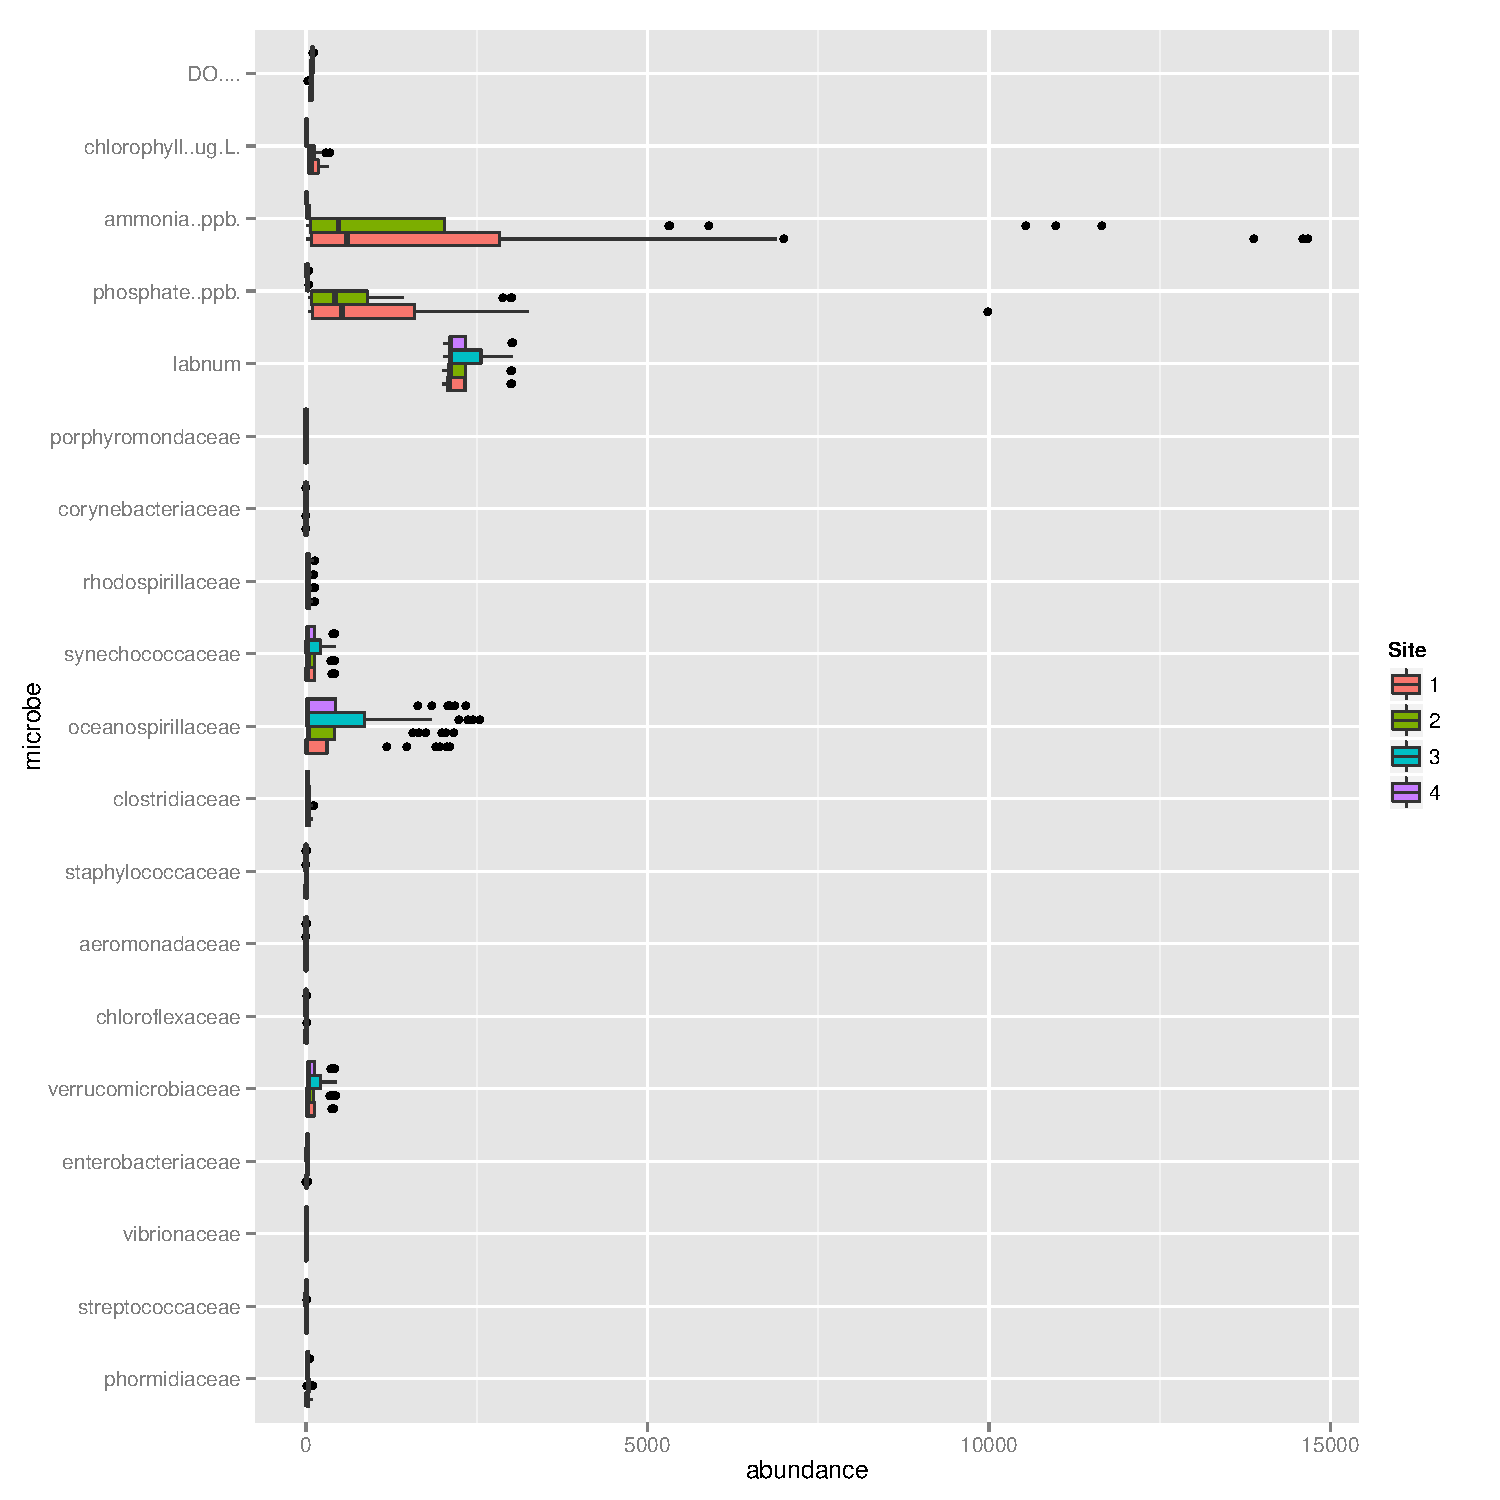
\includegraphics[width=.85\linewidth]{figure/chunk10iv-1} 

\end{knitrout}
\end{frame}  


\begin{frame}[fragile]
  \frametitle{Finding Outliers}
  \framesubtitle{Interquartile range}
  \begin{block}{Finding Outliers}
  \begin{itemize}
  \item Outliers are defined 1.5 times the interquartile range above the upper quartile
  \item Assume that  rows 12 and 14 in phosphate are errors as the 9 is typed twice
  \item Still issues with ammonia to explore
  \end{itemize} 
   \end{block}   
\begin{knitrout}
\definecolor{shadecolor}{rgb}{0.969, 0.969, 0.969}\color{fgcolor}\begin{kframe}
\begin{alltt}
 \hlstd{phosphate}\hlkwb{<-}\hlstd{table4[,}\hlstr{"phosphate..ppb."}\hlstd{]}
 \hlstd{upper.limit} \hlkwb{<-} \hlkwd{quantile}\hlstd{(phosphate)[}\hlnum{4}\hlstd{]} \hlopt{+} \hlnum{1.5}\hlopt{*}\hlkwd{IQR}\hlstd{(phosphate)}
 \hlstd{lower.limit} \hlkwb{<-} \hlkwd{quantile}\hlstd{(phosphate)[}\hlnum{2}\hlstd{]} \hlopt{-} \hlnum{1.5}\hlopt{*}\hlkwd{IQR}\hlstd{(phosphate)}
 \hlcom{#table4[phosphate> upper.limit,c("Site","phosphate..ppb.")]}
\end{alltt}
\end{kframe}
\end{knitrout}
\end{frame}

\begin{frame}[fragile]
  \frametitle{Reshaping Tables}
  \framesubtitle{Finding Outliers}
  \begin{block}{Removing Outliers}
   \end{block}   
% latex table generated in R 3.1.2 by xtable 1.7-4 package
% Wed Sep 30 19:56:02 2015
\begin{table}[ht]
\centering
\begin{tabular}{rlr}
  \hline
 & Site & phosphate..ppb. \\ 
  \hline
1 & 1 & 3020.00 \\ 
  2 & 1 & 3253.00 \\ 
  3 & 1 & 3169.00 \\ 
  12 & 1 & 9982.00 \\ 
  14 & 1 & 9982.00 \\ 
  16 & 1 & 1542.00 \\ 
   \hline
\end{tabular}
\end{table}

\begin{knitrout}
\definecolor{shadecolor}{rgb}{0.969, 0.969, 0.969}\color{fgcolor}\begin{kframe}
\begin{alltt}
\hlstd{table4[}\hlnum{12}\hlstd{,}\hlstr{"phosphate..ppb."}\hlstd{]}\hlkwb{<-}\hlnum{982}
\hlstd{table4[}\hlnum{14}\hlstd{,}\hlstr{"phosphate..ppb."}\hlstd{]}\hlkwb{<-}\hlnum{982}
\end{alltt}
\end{kframe}
\end{knitrout}
\end{frame}

\begin{frame}[fragile]
  \frametitle{Outliers check}
  \framesubtitle{ Redo the boxplot}
  \begin{block}{Look again ggplot}
  \end{block}

\begin{knitrout}
\definecolor{shadecolor}{rgb}{0.969, 0.969, 0.969}\color{fgcolor}\begin{kframe}


{\ttfamily\noindent\color{warningcolor}{\#\# Warning: Removed 24 rows containing non-finite values (stat\_boxplot).}}\end{kframe}
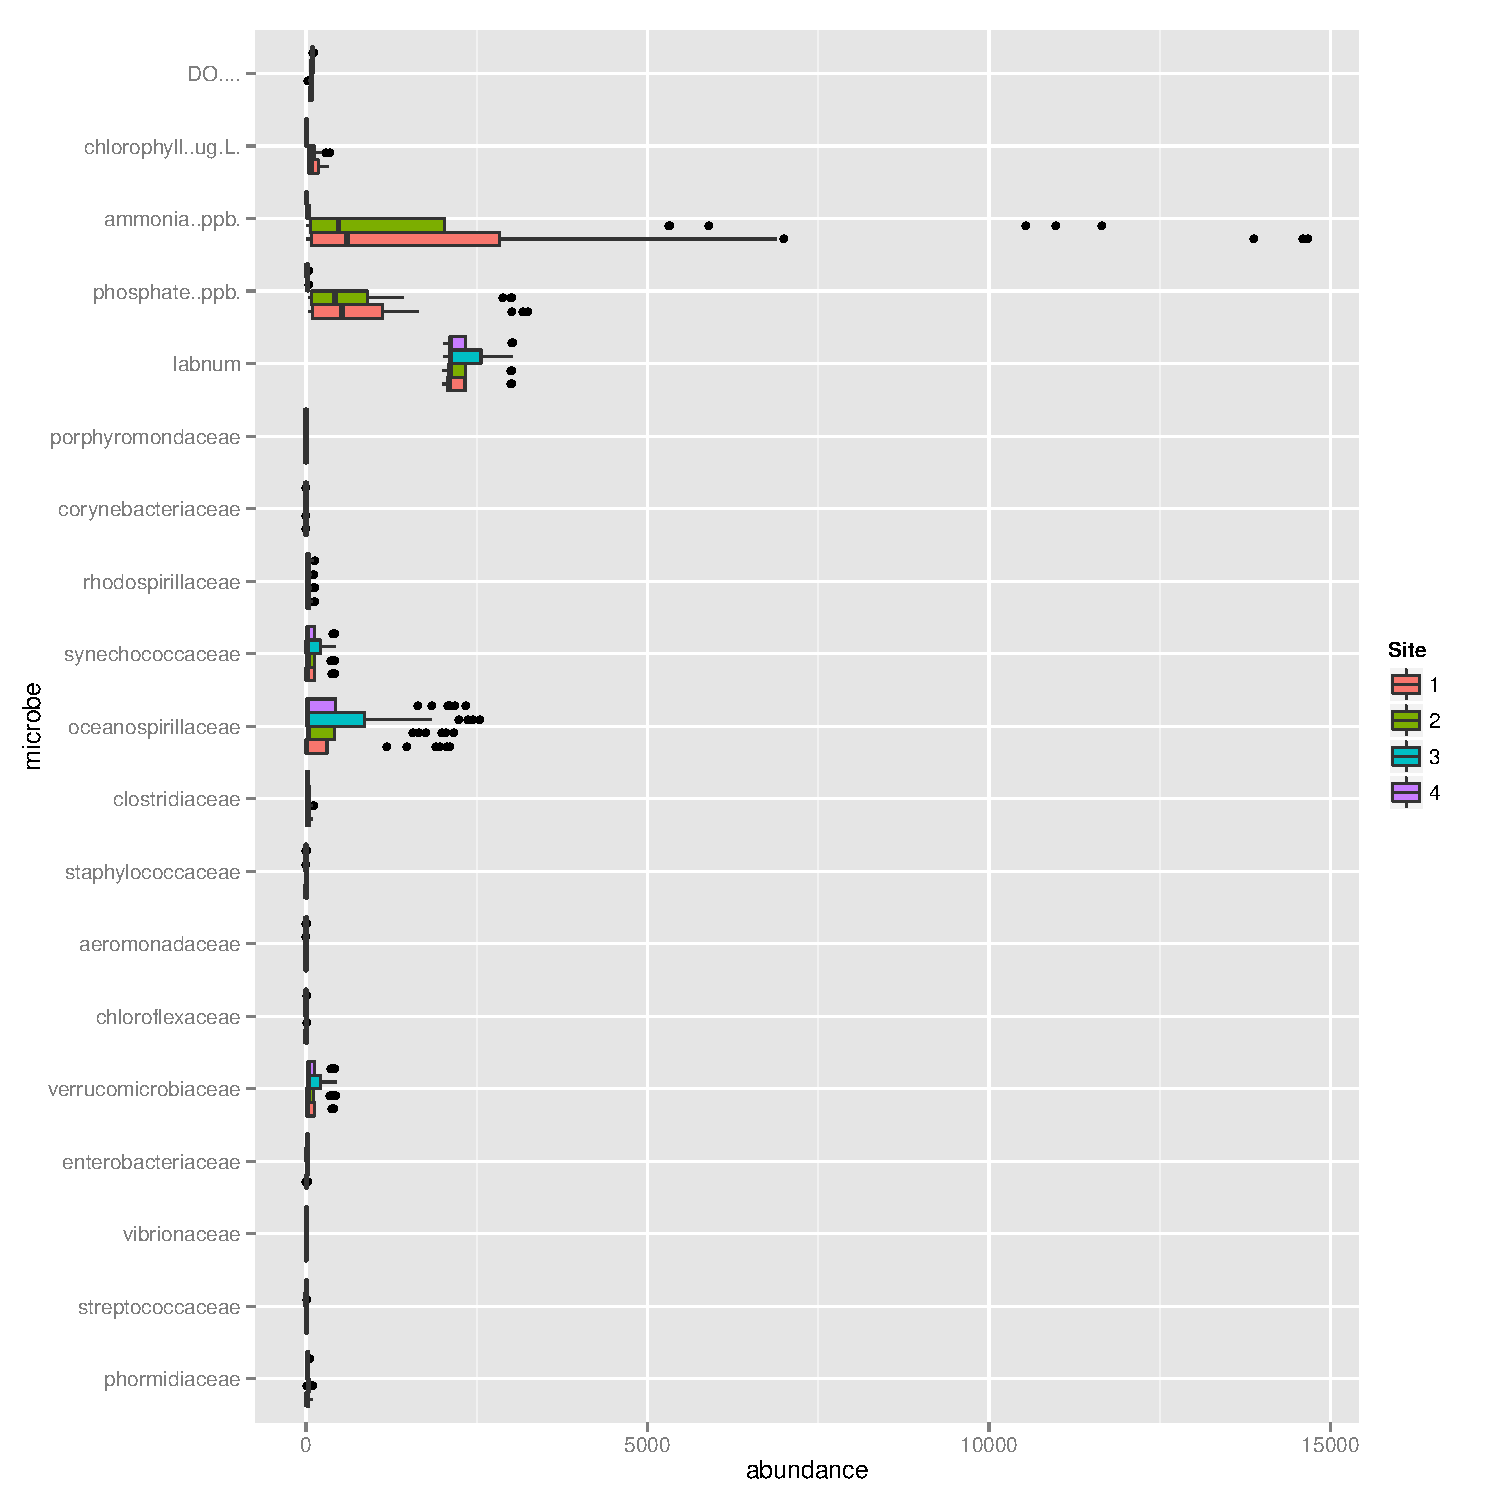
\includegraphics[width=.85\linewidth]{figure/chunk10viii-1} 

\end{knitrout}
\end{frame} 

\begin{frame}[fragile]
  \frametitle{R package}
  \framesubtitle{RQLlite}
  \begin{block}{RSQLite}
  \begin{itemize}
  \item Suppose merge is not enough? I know about SQL and want to do joins
  \item Install RSQLite
  \item We also need to install DBI
  \end{itemize}
  \end{block}
\begin{knitrout}
\definecolor{shadecolor}{rgb}{0.969, 0.969, 0.969}\color{fgcolor}\begin{kframe}


{\ttfamily\noindent\itshape\color{messagecolor}{\#\# Loading required package: RSQLite}}\end{kframe}
\end{knitrout}

\begin{knitrout}
\definecolor{shadecolor}{rgb}{0.969, 0.969, 0.969}\color{fgcolor}\begin{kframe}
\begin{alltt}
 \hlstd{db} \hlkwb{<-} \hlkwd{dbConnect}\hlstd{(}\hlkwd{SQLite}\hlstd{(),} \hlkwc{dbname}\hlstd{=}\hlstr{"Test.sqlite"}\hlstd{)}
\hlcom{#getConfig()$staged.queries}
\hlcom{# sqldf(attach "Test1.sqlite" as new)}
\hlkwd{dbBegin}\hlstd{(db)}
\end{alltt}
\begin{verbatim}
## [1] TRUE
\end{verbatim}
\begin{alltt}
\hlkwd{dbWriteTable}\hlstd{(db,}\hlstr{"table1"}\hlstd{,table1t,}\hlkwc{overwrite}\hlstd{=}\hlnum{TRUE}\hlstd{)}
\end{alltt}
\begin{verbatim}
## [1] TRUE
\end{verbatim}
\begin{alltt}
\hlkwd{dbReadTable}\hlstd{(db,}\hlstr{"table1"}\hlstd{)}
\end{alltt}
\begin{verbatim}
##                  Group  Site Sample.ID   Rep phormidiaceae
## X2        Contaminated     1     10000     1         24872
## X3        Contaminated     1     10001     2         24872
## X4        Contaminated     1     10002     3          5822
## X5        Contaminated     2     10003     1          7538
## X6        Contaminated     2     10004     2          7201
## X7        Contaminated     2     10005     3          7538
## X8        Contaminated     1     10006     1          8467
## X9        Contaminated     1     10007     2          7340
## X10       Contaminated     1     10008     3          8467
## X11       Contaminated     2     10000     1          2000
## X12       Contaminated     2     10001     2          2083
## X13       Contaminated     2     10002     3          1899
## X14       Contaminated     1     10003     1          1947
## X15       Contaminated     1     10004     2          2733
## X16       Contaminated     1     10005     3          2385
## X17       Contaminated     2     10006     1           800
## X18       Contaminated     2     10007     2           738
## X19       Contaminated     2     10008     3           800
## X20       Contaminated     1     10003     1           200
## X21       Contaminated     1     10004     2           189
## X22       Contaminated     1     10005     3           271
## X23       Contaminated     2     10006     1            46
## X24       Contaminated     2     10007     2            62
## X25       Contaminated     2     10008     3            94
## X26       Contaminated     3     10009     1            24
## X27            Control     3     10010     2            64
## X28            Control     3     10011     3            21
## X29            Control     4     10012     1            56
## X30            Control     4     10013     2            27
## X31            Control     4     10014     3            53
## X32            Control     3     10015     1           115
## X33            Control     3     10016     2            97
## X34            Control     3     10017     3            45
## X35            Control     4     10009     1            33
## X36            Control     4     10010     2            51
## X37            Control     4     10011     3            47
## X38            Control     3     10012     1           105
## X39            Control     3     10013     2            72
## X40            Control     3     10014     3           115
## X41            Control     4     10015     1            18
## X42            Control     4     10016     2            54
## X43            Control     4     10017     3            33
## X44            Control     3     10012     1            36
## X45            Control     3     10013     2            58
## X46            Control     3     10014     3            36
## X47            Control     4     10015     1            60
## X48            Control     4     10016     2           164
## X49            Control     4     10017     3            79
## rowNames         FALSE FALSE     FALSE F1LSE         FALSE
## transpose         TRUE  TRUE      TRUE  TRUE          TRUE
##           streptococcaceae vibrionaceae enterobacteriaceae
## X2                      11           33                131
## X3                       7           40                200
## X4                      14           40                200
## X5                       8           95                151
## X6                      10           83                140
## X7                       8           95                151
## X8                       5           29                132
## X9                       5           51                168
## X10                      5           29                132
## X11                     10           34                 97
## X12                     17           38                 91
## X13                     27           31                 51
## X14                      0            0                  2
## X15                      1            0                  1
## X16                      0            0                  2
## X17                     26           33                 34
## X18                     22           58                 42
## X19                     26           33                 34
## X20                      6            5                 39
## X21                      2            3                 23
## X22                      5            1                 39
## X23                      3            9                 55
## X24                      1            5                 95
## X25                      3            0                 55
## X26                      2            6                 36
## X27                      3            3                 36
## X28                      0            4                 30
## X29                      1           30                 79
## X30                      5            9                129
## X31                      1            1                124
## X32                      0           10                 52
## X33                      4            6                 13
## X34                      0            2                  9
## X35                      4            4                 11
## X36                      0           10                 41
## X37                      0            3                 29
## X38                     10           39                288
## X39                     10           29                413
## X40                     12           34                481
## X41                      5            2                 43
## X42                      3            5                 50
## X43                      4            5                 86
## X44                     10            4                 28
## X45                     12            1                 28
## X46                      1            0                 44
## X47                      4            7                 48
## X48                      2           11                111
## X49                      3            5                 88
## rowNames             FALSE        FALSE              FALSE
## transpose             TRUE         TRUE               TRUE
##           verrucomicrobiaceae chloroflexaceae aeromonadaceae
## X2                        977             351             20
## X3                       1500             246             76
## X4                        844             246             76
## X5                       1006              41              1
## X6                       1112              83              6
## X7                       1195              41              0
## X8                       1805              23              0
## X9                       1906              28              0
## X10                      1902              23              0
## X11                      1244              40              1
## X12                      1933              40              1
## X13                      1244              80              0
## X14                       251               1              0
## X15                       271               0              1
## X16                       299               0              0
## X17                      1348             209              1
## X18                      3612             205              0
## X19                      1348             209              3
## X20                       176               1              0
## X21                       211               0              3
## X22                       183               1              0
## X23                       544               0              9
## X24                       611               1              0
## X25                       544               0              1
## X26                       471               0              0
## X27                       500               0              1
## X28                       541               0              0
## X29                      1405               3              1
## X30                      1678               1              1
## X31                      1360               0              0
## X32                      1590               0              0
## X33                       398               0              0
## X34                       195               1              0
## X35                      1213               7              2
## X36                      3461              12              1
## X37                      1688               3              0
## X38                       590               1              1
## X39                       598               0              0
## X40                       639               1              0
## X41                       949               0              0
## X42                       974               0              0
## X43                       662               0              0
## X44                       267               0              0
## X45                       249               2              0
## X46                       337               0              0
## X47                       625               0              0
## X48                       886               0              0
## X49                       791               0              0
## rowNames                FALSE           FALSE          FALSE
## transpose                TRUE            TRUE           TRUE
##           staphylococcaceae clostridiaceae oceanospirillaceae
## X2                      115            274               1438
## X3                      342            288               1789
## X4                      342            258               1789
## X5                        4            365                  5
## X6                        9            365                  2
## X7                        4            365                  9
## X8                        1            643                 14
## X9                        1            941                 14
## X10                       1            711                 14
## X11                       0            204                 93
## X12                       0            229                 72
## X13                       0            285                 93
## X14                       0              8               1080
## X15                       0             12               1633
## X16                       1             12               1080
## X17                       4            400                747
## X18                       7            733                636
## X19                       2            299                747
## X20                       1             76                256
## X21                       0             63                263
## X22                       2             85                256
## X23                       1            136                284
## X24                      20            643                293
## X25                       1            136                293
## X26                       0             31                189
## X27                       1             59                510
## X28                       0             42                215
## X29                       0            143               2096
## X30                       0            124                834
## X31                       0            100                426
## X32                       0             34                263
## X33                       0             33               1095
## X34                       0             18                523
## X35                       0             96                273
## X36                       0            100               1432
## X37                       0             74                330
## X38                       1            119               4584
## X39                       1            181               3811
## X40                       0            202               3165
## X41                       0             38                380
## X42                       0             29                548
## X43                       0             56                403
## X44                       0             62                394
## X45                       0             58                311
## X46                       0             66                376
## X47                       0             66                773
## X48                       0            167               1778
## X49                       0             40               1289
## rowNames              FALSE          FALSE              FALSE
## transpose              TRUE           TRUE               TRUE
##           synechococcaceae rhodospirillaceae corynebacteriaceae
## X2                     471              1267                  0
## X3                     498              1597                  0
## X4                     692              1844                  0
## X5                      20                70                  0
## X6                      20                82                  0
## X7                      48                70                  0
## X8                      27                97                  0
## X9                      83                97                  0
## X10                     27                97                  0
## X11                     61               579                  0
## X12                     61               603                  0
## X13                     61               579                  0
## X14                    245              2245                  0
## X15                    245              2001                  0
## X16                    142              2834                  0
## X17                     95              1432                  0
## X18                     70              1834                  0
## X19                     95              1432                  0
## X20                    101               786                  0
## X21                    104               844                  0
## X22                    101               826                  0
## X23                     65              1833                  0
## X24                     53              2528                  0
## X25                     65              2999                  0
## X26                     67               568                  0
## X27                    128              1877                  0
## X28                    152               582                  0
## X29                    769              1699                  0
## X30                    954              3145                  0
## X31                    555              1171                  0
## X32                     45               323                  0
## X33                    164               911                  0
## X34                    513               485                  0
## X35                     75               732                  0
## X36                    414              3101                  0
## X37                    298              1262                  0
## X38                    807              3586                  0
## X39                   1916              5757                  0
## X40                   1120              4168                  0
## X41                    276               821                  0
## X42                    394               489                  0
## X43                    498               611                  0
## X44                    212              1001                  0
## X45                    301               889                  0
## X46                    330               943                  0
## X47                    521              1300                  0
## X48                   1220              3013                  0
## X49                    383              1255                  0
## rowNames             FALSE             FALSE              FALSE
## transpose             TRUE              TRUE               TRUE
##           porphyromondaceae
## X2                        0
## X3                        0
## X4                        0
## X5                        0
## X6                        0
## X7                        0
## X8                        0
## X9                        0
## X10                       0
## X11                       0
## X12                       0
## X13                       0
## X14                       0
## X15                       0
## X16                       0
## X17                       0
## X18                       0
## X19                       0
## X20                       0
## X21                       0
## X22                       0
## X23                       0
## X24                       0
## X25                       0
## X26                       0
## X27                       0
## X28                       0
## X29                       0
## X30                       0
## X31                       0
## X32                       0
## X33                       0
## X34                       0
## X35                       0
## X36                       0
## X37                       0
## X38                       0
## X39                       0
## X40                       0
## X41                       0
## X42                       0
## X43                       0
## X44                       0
## X45                       0
## X46                       0
## X47                       0
## X48                       0
## X49                       0
## rowNames              FALSE
## transpose              TRUE
\end{verbatim}
\begin{alltt}
\hlkwd{dbListFields}\hlstd{(db,}\hlstr{"table1"}\hlstd{)}
\end{alltt}
\begin{verbatim}
##  [1] "row_names"           "Group"               "Site"               
##  [4] "Sample ID"           "Rep"                 "phormidiaceae"      
##  [7] "streptococcaceae"    "vibrionaceae"        "enterobacteriaceae" 
## [10] "verrucomicrobiaceae" "chloroflexaceae"     "aeromonadaceae"     
## [13] "staphylococcaceae"   "clostridiaceae"      "oceanospirillaceae" 
## [16] "synechococcaceae"    "rhodospirillaceae"   "corynebacteriaceae" 
## [19] "porphyromondaceae"
\end{verbatim}
\begin{alltt}
\hlkwd{dbListTables}\hlstd{(db)}
\end{alltt}
\begin{verbatim}
## [1] "table1"
\end{verbatim}
\begin{alltt}
\hlkwd{dbGetQuery}\hlstd{(db,} \hlstr{"SELECT * from table1"}\hlstd{)}
\end{alltt}
\begin{verbatim}
##    row_names        Group  Site Sample ID   Rep phormidiaceae
## 1         X2 Contaminated     1     10000     1         24872
## 2         X3 Contaminated     1     10001     2         24872
## 3         X4 Contaminated     1     10002     3          5822
## 4         X5 Contaminated     2     10003     1          7538
## 5         X6 Contaminated     2     10004     2          7201
## 6         X7 Contaminated     2     10005     3          7538
## 7         X8 Contaminated     1     10006     1          8467
## 8         X9 Contaminated     1     10007     2          7340
## 9        X10 Contaminated     1     10008     3          8467
## 10       X11 Contaminated     2     10000     1          2000
## 11       X12 Contaminated     2     10001     2          2083
## 12       X13 Contaminated     2     10002     3          1899
## 13       X14 Contaminated     1     10003     1          1947
## 14       X15 Contaminated     1     10004     2          2733
## 15       X16 Contaminated     1     10005     3          2385
## 16       X17 Contaminated     2     10006     1           800
## 17       X18 Contaminated     2     10007     2           738
## 18       X19 Contaminated     2     10008     3           800
## 19       X20 Contaminated     1     10003     1           200
## 20       X21 Contaminated     1     10004     2           189
## 21       X22 Contaminated     1     10005     3           271
## 22       X23 Contaminated     2     10006     1            46
## 23       X24 Contaminated     2     10007     2            62
## 24       X25 Contaminated     2     10008     3            94
## 25       X26 Contaminated     3     10009     1            24
## 26       X27      Control     3     10010     2            64
## 27       X28      Control     3     10011     3            21
## 28       X29      Control     4     10012     1            56
## 29       X30      Control     4     10013     2            27
## 30       X31      Control     4     10014     3            53
## 31       X32      Control     3     10015     1           115
## 32       X33      Control     3     10016     2            97
## 33       X34      Control     3     10017     3            45
## 34       X35      Control     4     10009     1            33
## 35       X36      Control     4     10010     2            51
## 36       X37      Control     4     10011     3            47
## 37       X38      Control     3     10012     1           105
## 38       X39      Control     3     10013     2            72
## 39       X40      Control     3     10014     3           115
## 40       X41      Control     4     10015     1            18
## 41       X42      Control     4     10016     2            54
## 42       X43      Control     4     10017     3            33
## 43       X44      Control     3     10012     1            36
## 44       X45      Control     3     10013     2            58
## 45       X46      Control     3     10014     3            36
## 46       X47      Control     4     10015     1            60
## 47       X48      Control     4     10016     2           164
## 48       X49      Control     4     10017     3            79
## 49  rowNames        FALSE FALSE     FALSE F1LSE         FALSE
## 50 transpose         TRUE  TRUE      TRUE  TRUE          TRUE
##    streptococcaceae vibrionaceae enterobacteriaceae verrucomicrobiaceae
## 1                11           33                131                 977
## 2                 7           40                200                1500
## 3                14           40                200                 844
## 4                 8           95                151                1006
## 5                10           83                140                1112
## 6                 8           95                151                1195
## 7                 5           29                132                1805
## 8                 5           51                168                1906
## 9                 5           29                132                1902
## 10               10           34                 97                1244
## 11               17           38                 91                1933
## 12               27           31                 51                1244
## 13                0            0                  2                 251
## 14                1            0                  1                 271
## 15                0            0                  2                 299
## 16               26           33                 34                1348
## 17               22           58                 42                3612
## 18               26           33                 34                1348
## 19                6            5                 39                 176
## 20                2            3                 23                 211
## 21                5            1                 39                 183
## 22                3            9                 55                 544
## 23                1            5                 95                 611
## 24                3            0                 55                 544
## 25                2            6                 36                 471
## 26                3            3                 36                 500
## 27                0            4                 30                 541
## 28                1           30                 79                1405
## 29                5            9                129                1678
## 30                1            1                124                1360
## 31                0           10                 52                1590
## 32                4            6                 13                 398
## 33                0            2                  9                 195
## 34                4            4                 11                1213
## 35                0           10                 41                3461
## 36                0            3                 29                1688
## 37               10           39                288                 590
## 38               10           29                413                 598
## 39               12           34                481                 639
## 40                5            2                 43                 949
## 41                3            5                 50                 974
## 42                4            5                 86                 662
## 43               10            4                 28                 267
## 44               12            1                 28                 249
## 45                1            0                 44                 337
## 46                4            7                 48                 625
## 47                2           11                111                 886
## 48                3            5                 88                 791
## 49            FALSE        FALSE              FALSE               FALSE
## 50             TRUE         TRUE               TRUE                TRUE
##    chloroflexaceae aeromonadaceae staphylococcaceae clostridiaceae
## 1              351             20               115            274
## 2              246             76               342            288
## 3              246             76               342            258
## 4               41              1                 4            365
## 5               83              6                 9            365
## 6               41              0                 4            365
## 7               23              0                 1            643
## 8               28              0                 1            941
## 9               23              0                 1            711
## 10              40              1                 0            204
## 11              40              1                 0            229
## 12              80              0                 0            285
## 13               1              0                 0              8
## 14               0              1                 0             12
## 15               0              0                 1             12
## 16             209              1                 4            400
## 17             205              0                 7            733
## 18             209              3                 2            299
## 19               1              0                 1             76
## 20               0              3                 0             63
## 21               1              0                 2             85
## 22               0              9                 1            136
## 23               1              0                20            643
## 24               0              1                 1            136
## 25               0              0                 0             31
## 26               0              1                 1             59
## 27               0              0                 0             42
## 28               3              1                 0            143
## 29               1              1                 0            124
## 30               0              0                 0            100
## 31               0              0                 0             34
## 32               0              0                 0             33
## 33               1              0                 0             18
## 34               7              2                 0             96
## 35              12              1                 0            100
## 36               3              0                 0             74
## 37               1              1                 1            119
## 38               0              0                 1            181
## 39               1              0                 0            202
## 40               0              0                 0             38
## 41               0              0                 0             29
## 42               0              0                 0             56
## 43               0              0                 0             62
## 44               2              0                 0             58
## 45               0              0                 0             66
## 46               0              0                 0             66
## 47               0              0                 0            167
## 48               0              0                 0             40
## 49           FALSE          FALSE             FALSE          FALSE
## 50            TRUE           TRUE              TRUE           TRUE
##    oceanospirillaceae synechococcaceae rhodospirillaceae
## 1                1438              471              1267
## 2                1789              498              1597
## 3                1789              692              1844
## 4                   5               20                70
## 5                   2               20                82
## 6                   9               48                70
## 7                  14               27                97
## 8                  14               83                97
## 9                  14               27                97
## 10                 93               61               579
## 11                 72               61               603
## 12                 93               61               579
## 13               1080              245              2245
## 14               1633              245              2001
## 15               1080              142              2834
## 16                747               95              1432
## 17                636               70              1834
## 18                747               95              1432
## 19                256              101               786
## 20                263              104               844
## 21                256              101               826
## 22                284               65              1833
## 23                293               53              2528
## 24                293               65              2999
## 25                189               67               568
## 26                510              128              1877
## 27                215              152               582
## 28               2096              769              1699
## 29                834              954              3145
## 30                426              555              1171
## 31                263               45               323
## 32               1095              164               911
## 33                523              513               485
## 34                273               75               732
## 35               1432              414              3101
## 36                330              298              1262
## 37               4584              807              3586
## 38               3811             1916              5757
## 39               3165             1120              4168
## 40                380              276               821
## 41                548              394               489
## 42                403              498               611
## 43                394              212              1001
## 44                311              301               889
## 45                376              330               943
## 46                773              521              1300
## 47               1778             1220              3013
## 48               1289              383              1255
## 49              FALSE            FALSE             FALSE
## 50               TRUE             TRUE              TRUE
##    corynebacteriaceae porphyromondaceae
## 1                   0                 0
## 2                   0                 0
## 3                   0                 0
## 4                   0                 0
## 5                   0                 0
## 6                   0                 0
## 7                   0                 0
## 8                   0                 0
## 9                   0                 0
## 10                  0                 0
## 11                  0                 0
## 12                  0                 0
## 13                  0                 0
## 14                  0                 0
## 15                  0                 0
## 16                  0                 0
## 17                  0                 0
## 18                  0                 0
## 19                  0                 0
## 20                  0                 0
## 21                  0                 0
## 22                  0                 0
## 23                  0                 0
## 24                  0                 0
## 25                  0                 0
## 26                  0                 0
## 27                  0                 0
## 28                  0                 0
## 29                  0                 0
## 30                  0                 0
## 31                  0                 0
## 32                  0                 0
## 33                  0                 0
## 34                  0                 0
## 35                  0                 0
## 36                  0                 0
## 37                  0                 0
## 38                  0                 0
## 39                  0                 0
## 40                  0                 0
## 41                  0                 0
## 42                  0                 0
## 43                  0                 0
## 44                  0                 0
## 45                  0                 0
## 46                  0                 0
## 47                  0                 0
## 48                  0                 0
## 49              FALSE             FALSE
## 50               TRUE              TRUE
\end{verbatim}
\begin{alltt}
\hlcom{#dbDisconnect(db)}
\end{alltt}
\end{kframe}
\end{knitrout}
\end{frame} 

\begin{frame}[fragile]
  \frametitle{R package}
  \framesubtitle{RQLlite}
  \begin{block}{RSQLite}
  \begin{itemize}
  \item Some links to RSQL ideas
\item \url{http://stackoverflow.com/questions/12307685/join-more-than-2-tables-in-r-using-rsqlite}
\item \url{https://support.rstudio.com/hc/en-us/articles/201057987-Quick-list-of-useful-R-packages}
\item \url{https://cran.rstudio.com/web/packages/dplyr/vignettes/introduction.html}
\end{itemize}
\end{block}
 \begin{lstlisting}
select coalesce(fileA,fileB),valA,valB
               from t1 LEFT OUTER JOIN t2 On t1.fileA= t2.fileB
UNION select coalesce(fileA,fileB),valA,valB
               from t2 LEFT OUTER JOIN t1 ON t1.fileA= t2.fileB
(CREATE TABLE all_files AS SELECT fileA FROM t1 UNION SELECT fileB from t2 UNION ...).             
 \end{lstlisting}

\end{frame}


\begin{frame}
  \frametitle{R package}
  \framesubtitle{svUnit}
     Another important component of TDD is refactoring and unit tests
  \begin{itemize}
     \item Refactoring \url{http://refactoring.com/}
     \item \url{http://www.r-bloggers.com/my-experience-of-learning-r-from-basic-graphs-to-performance-tuning/}
     \item TDD in R \url{http://www.slideserve.com/andrew/test-driven-development-in-r}
     \item Version Control tortiseSVN {\url http://tortoisesvn.net/}
     \item GitHub \url{https://github.com/}
  \end{itemize}
\end{frame}


%%%%%%%%%%%%%%%%%%%%%%%%%


%\section*[Dropping Columns]{Cleaning things up}
\section*{Cleaning things up}
\begin{frame}[fragile]
  \frametitle{Dropping row and columns}
  \framesubtitle{Dropping selected variables}
  \begin{block}{Dropping Row and Columns with too many NAs}  
  \end{block}
\begin{lstlisting}
numNAs_inData4_rows <- apply(rawData4, 1, function(z) sum(is.na(z))) 
numNAs_inData4_col <- apply(table4, 2, function(z) sum(is.na(z))) # count NAs in Data4
lessThan20 <- table4[!(numNAs_inData4_rows > 20),]	   #only select the rows contain less Than 20 NAs
lessThan20col <- table4[,!(numNAs_inData4_col > 20)]
\end{lstlisting}
\end{frame}

\begin{frame}[fragile]
  \frametitle{Dropping row and columns}
  \framesubtitle{Dropping selected variables}

\begin{block}{Tidy Data}
In tidy data:
\begin{itemize}
\item Each variable forms a column.
\item Each observation forms a row.
\item Each type of observational unit forms a table.
\item \url{https://cran.r-project.org/web/packages/tidyr/vignettes/tidy-data.html}
\item \url{http://pj.freefaculty.org/R/Rtips.html#toc-Subsection-1.11}
\end{itemize}
\end{block}
 

\begin{block}{Spit out the dates and numbers}
\end{block}
\begin{lstlisting}
dates4<-table4[,c(5,6)]
abundance<-table4[,c(7:25)]
\end{lstlisting}
\end{frame}


\begin{frame}[fragile]
  \frametitle{Adding a new column}
  \framesubtitle{Calculating the number of days}
  %Using the $is.Date$ command
  \begin{block}{Calculating the number of days}
  We can just subtract as.Date fields
  \end{block}
\begin{knitrout}
\definecolor{shadecolor}{rgb}{0.969, 0.969, 0.969}\color{fgcolor}\begin{kframe}
\begin{alltt}
\hlstd{dates4}\hlkwb{<-}\hlstd{table4[,}\hlkwd{c}\hlstd{(}\hlnum{5}\hlstd{,}\hlnum{6}\hlstd{)]}
\hlstd{abundance}\hlkwb{<-}\hlstd{table4[,}\hlkwd{c}\hlstd{(}\hlnum{7}\hlopt{:}\hlnum{25}\hlstd{)]}
 \hlstd{days}\hlkwb{<-}\hlstd{dates4[,}\hlnum{2}\hlstd{]}\hlopt{-}\hlstd{dates4[,}\hlnum{1}\hlstd{]}
\end{alltt}
\end{kframe}
\end{knitrout}
  
\end{frame}


%\section*[Normalizeing]{Setting the Relative Abundance}
\section*{Setting the relative abundance}
\begin{frame}[fragile]
  \frametitle{Setting the relative abundance}
  \framesubtitle{Normalizing data}
  \begin{block}{sapply}
  \begin{itemize}
  \item Also known as centring the data
  \item Ecological percentage of the sum of the variables 
  \item We an use sweep to centre the data
  \item $options(digits=1)$ Just to make things pretty
 % \item What about divide by 0
  \end{itemize}
  \end{block}
  \begin{lstlisting}
sweepOutContinu<-sweep(abundance,2,apply(abundance,2,min,na.rm=TRUE))	
afterSweepContinu<-sweep(sweepOutContinu,2,apply(sweepOutContinu,2,max,na.rm=TRUE),"/") 
table5<-cbind(table4[,c(1:6)],afterSweepContinu,days)
options(digits=1)
sweep(abundance, 2, colSums(abundance), FUN="/")
scale(abundance, center=FALSE, scale=colSums(abundance))
 \end{lstlisting}

\end{frame}



\begin{frame}[fragile]
  \frametitle{Now let's have some fun}
  \framesubtitle{Graphics in R}
\begin{block}{R has nice graphs}
\begin{itemize}
\item A graphical output
\item \url{http://rcharts.io/gallery/}
\item R Graph gallery currently down try \url{http://rgraphgallery.blogspot.com/}
%  Titles on R plots
\item A reference on where to go R thumbnails 
\item ggplot2 (scatter plot of 2 var and then 3 plots)
\item To create a correlation heat map
\end{itemize}
\end{block}  
\begin{lstlisting}
 library(corrplot)
 abuncor<-cor(t5lessThan20col[,c(6:22)])
 require(corrplot)
 corrplot(abuncor, method = "circle")
\end{lstlisting} 

\begin{knitrout}
\definecolor{shadecolor}{rgb}{0.969, 0.969, 0.969}\color{fgcolor}\begin{kframe}
\begin{verbatim}
## [1] 23
\end{verbatim}


{\ttfamily\noindent\itshape\color{messagecolor}{\#\# Loading required package: corrplot}}\end{kframe}
\end{knitrout}

\end{frame}
 
 \begin{frame}[fragile]
  \frametitle{Now let's have some fun}
  \framesubtitle{Making a heat map}
\begin{block}{A heat map}
\end{block}
%<<boring-plots, fig.width=5, fig.height=5, out.width='.45\\linewidth', fig.show='hold'>>=
\begin{knitrout}
\definecolor{shadecolor}{rgb}{0.969, 0.969, 0.969}\color{fgcolor}
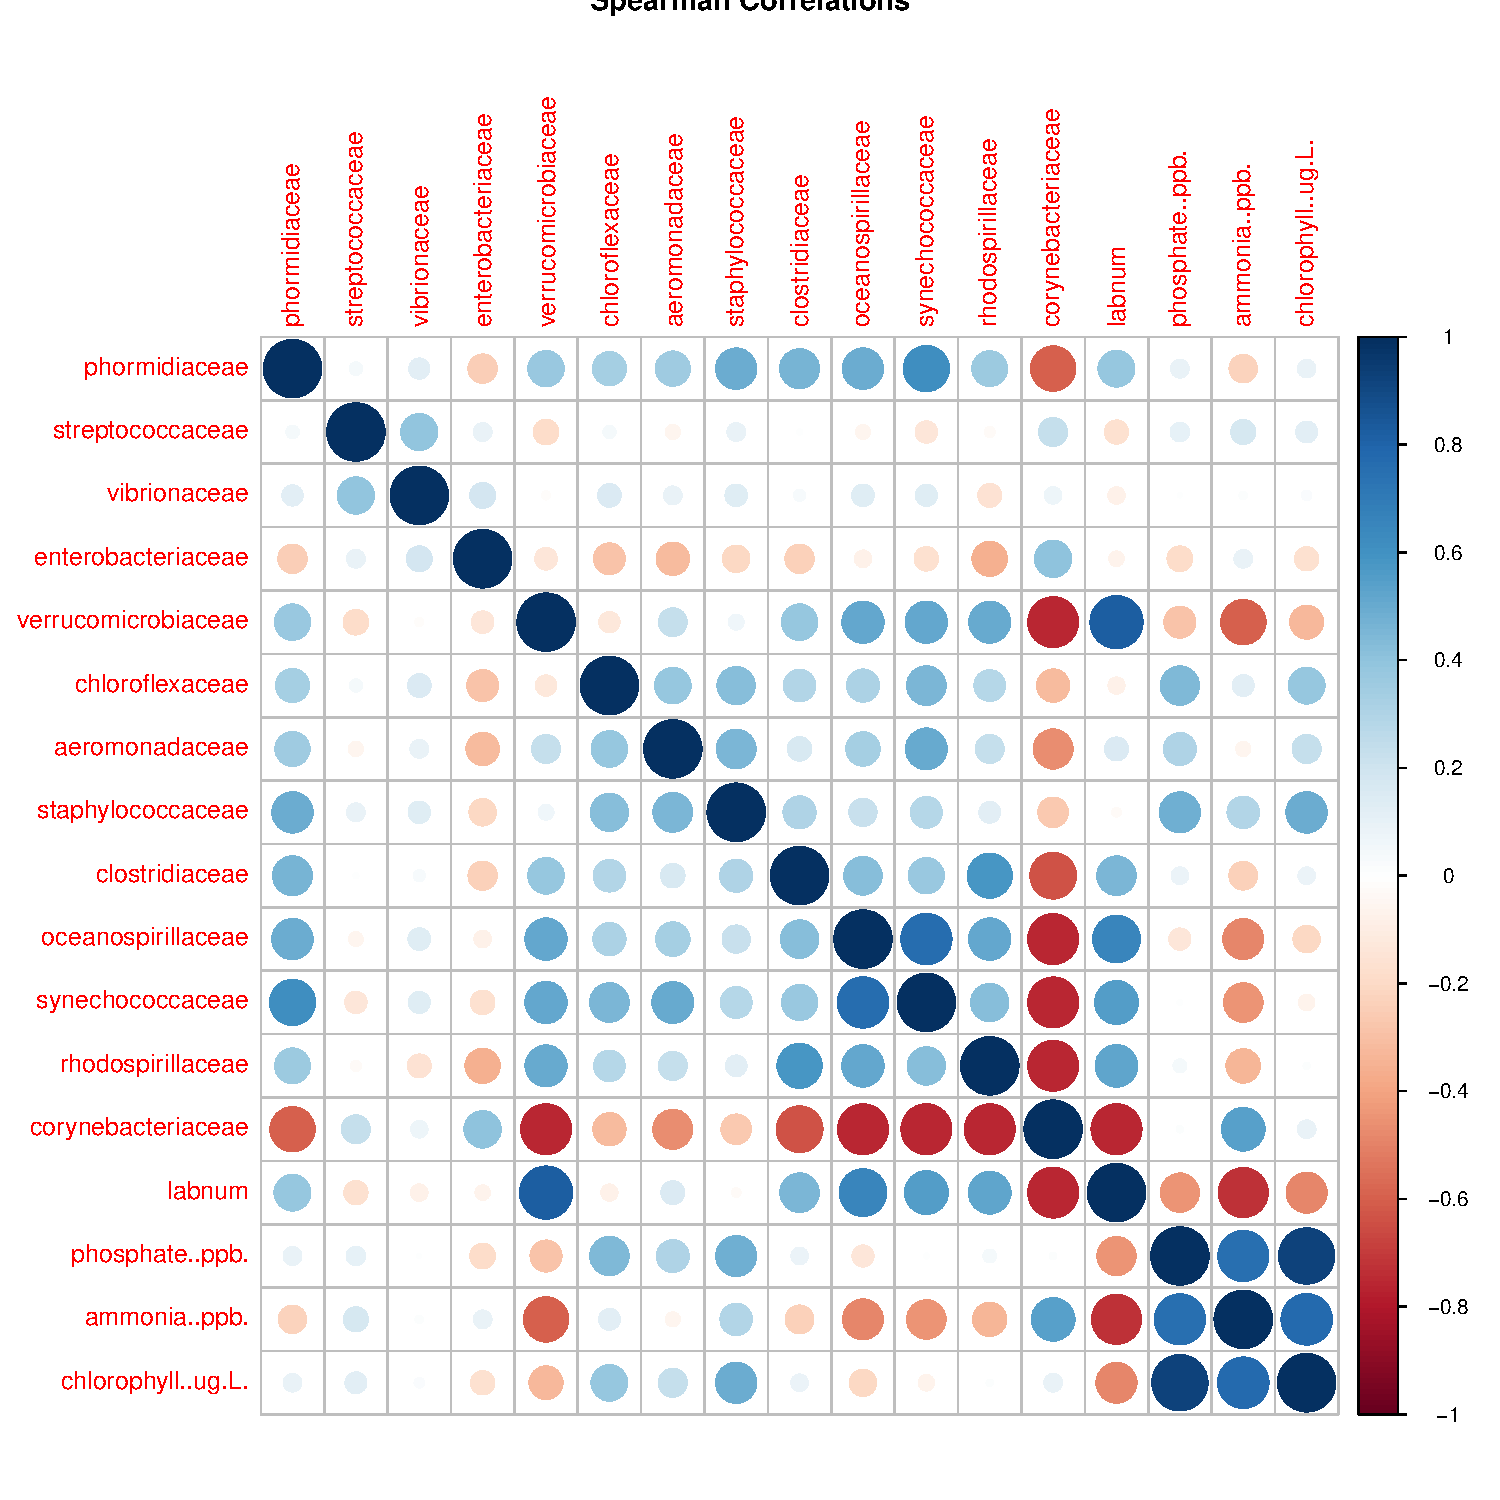
\includegraphics[width=.85\linewidth]{figure/chunk12i-1} 

\end{knitrout}
\end{frame}
%http://www.cookbook-r.com/Graphs/Plotting_distributions_(ggplot2)/


 \begin{frame}[fragile]
  \frametitle{Simple Tests}
  \framesubtitle{ttests}
\begin{block}{t tests}
There are many $t-tests$ available in R
\url{http://www.statmethods.net/stats/ttest.html}
\end{block}

\begin{knitrout}
\definecolor{shadecolor}{rgb}{0.969, 0.969, 0.969}\color{fgcolor}\begin{kframe}
\begin{alltt}
\hlcom{# independent 2-group t-test}
\hlkwd{t.test}\hlstd{(t5lessThan20col[,}\hlnum{12}\hlstd{],t5lessThan20col[,}\hlnum{8}\hlstd{])}
\end{alltt}
\begin{verbatim}
## 
## 	Welch Two Sample t-test
## 
## data:  t5lessThan20col[, 12] and t5lessThan20col[, 8]
## t = -3.4052, df = 180.441, p-value = 0.0008149
## alternative hypothesis: true difference in means is not equal to 0
## 95 percent confidence interval:
##  -0.20589367 -0.05481872
## sample estimates:
## mean of x mean of y 
## 0.2725146 0.4028708
\end{verbatim}
\end{kframe}
\end{knitrout}
\end{frame}

\begin{frame}
  \frametitle{What next}
  \framesubtitle{Proposed future talks}
  \begin{block}{Help is on the way}
  \begin{itemize}
  \item Parameterized Complexity Research Unit (PCRU) PhD students
  \item PhD student in Bioinformatics from Central South Uni
  \end{itemize}
  \end{block}
  \begin{block}{Your feedback on some ideas}
  \begin{itemize}
  \item Using Sweave or Knitr
  \item Advanced Data Cleaning 
  \item Network Centric data analysis
  \end{itemize}
  \end{block}
\end{frame}

\begin{frame}
  \frametitle{Resources}
  \framesubtitle{If you want to improve this style}
  \begin{thebibliography}{10}

  \beamertemplatearticlebibitems
%https://www.getdatajoy.com/
  \bibitem{beamer-homepage}
    LaTeX Beamer
    \newblock {\tt http://latex-beamer.sourceforge.net/}

  \bibitem{}
    Sharelatex Site % a link to my slides
    \newblock {\tt https://www.sharelatex.com}
  \bibitem{}
    A Data Cleaning Mooc % a link to my slides
    \newblock {\tt https://www.sharelatex.com}    
%    https://www.coursera.org/course/repdata
  \end{thebibliography}
\end{frame}

\begin{frame}[fragile]
  \frametitle{R Packages Used}
  \framesubtitle{Session Info}
\begin{block}{Output of sessionInfo}
\end{block}
\begin{knitrout}
\definecolor{shadecolor}{rgb}{0.969, 0.969, 0.969}\color{fgcolor}\begin{kframe}
\begin{alltt}
\hlkwd{sessionInfo}\hlstd{()}
\end{alltt}
\begin{verbatim}
## R version 3.1.2 (2014-10-31)
## Platform: x86_64-apple-darwin13.4.0 (64-bit)
## 
## locale:
## [1] C
## 
## attached base packages:
## [1] methods   stats     graphics  grDevices utils     datasets  base     
## 
## other attached packages:
##  [1] corrplot_0.73  RSQLite_1.0.0  DBI_0.3.1      ggplot2_1.0.0 
##  [5] reshape2_1.4.1 plyr_1.8.1     stringr_0.6.2  xtable_1.7-4  
##  [9] xlsx_0.5.7     xlsxjars_0.6.1 rJava_0.9-7    knitr_1.11    
## 
## loaded via a namespace (and not attached):
##  [1] MASS_7.3-39      Rcpp_0.11.5      colorspace_1.2-6 digest_0.6.8    
##  [5] evaluate_0.7.2   formatR_1.2      grid_3.1.2       gtable_0.1.2    
##  [9] highr_0.5        labeling_0.3     munsell_0.4.2    proto_0.3-10    
## [13] scales_0.2.4     tools_3.1.2
\end{verbatim}
\begin{alltt}
\hlcom{#  packages_in_use <- c( sessionInfo()$basePkgs, names( sessionInfo()$loadedOnly ) )}
\hlcom{#the_citations_list <- lapply( X=packages_in_use, FUN=citation)}
\hlcom{#the_citations_list}
\end{alltt}
\end{kframe}
\end{knitrout}
\end{frame}

%\frame{
%  \vspace{2cm}
%  {\huge Questions ?}
%
%  \vspace{3cm}
%  \begin{flushright}
%    Peter Shaw
%
%    \structure{\footnotesize{peter.shaw@cdu.edu.au}}
%  \end{flushright}
%}


%You can type R commands in your \LaTeX{} document and they will be properly run and the output printed in the document.

%<<chunk1>>=
%# Create a sequence of numbers
%X = 2:10
%
%# Display basic statistical measures
%summary(X)
%
%@
%--------------------------------------------------------------------------------

%So, the mean of the data is $mean(X)$ %Inline command


%\clearpage
%Plots
%--------------------------------------------------------------------------------
%<<plot1, fig.pos="t", fig.height=4, fig.width=4, fig.cap="First plot">>=

%xdata = read.csv(file="data.txt", head=TRUE,sep=" ")

%hist(xdata$data, main="ShareLaTeX histogram", xlab="Data")

%@
%--------------------------------------------------------------------------------

%The figure \ref{fig:plot1} is simple histogram.

%\clearpage

%The chunk below will not be printed

%R code imported from external file
%--------------------------------------------------------------------------------
%<<echo=FALSE, cache=FALSE>>=
%read_chunk("mycode.R")
%@

%The code must show up here

%<<myrcode2>>=

%@
%--------------------------------------------------------------------------------


%\frame{
%  \vspace{2cm}
%  {\huge Questions ?}

%  \vspace{3cm}
%  \begin{flushright}
%    Peter Shaw

%    \structure{\footnotesize{peter.shaw@cdu.edu.au}}
%  \end{flushright}
%}
\end{document}
